% Options for packages loaded elsewhere
\PassOptionsToPackage{unicode}{hyperref}
\PassOptionsToPackage{hyphens}{url}
\PassOptionsToPackage{dvipsnames,svgnames,x11names}{xcolor}
\documentclass[
]{article}
\usepackage{xcolor}
\usepackage[margin=1in]{geometry}
\usepackage{amsmath,amssymb}
\setcounter{secnumdepth}{5}
\usepackage{iftex}
\ifPDFTeX
  \usepackage[T1]{fontenc}
  \usepackage[utf8]{inputenc}
  \usepackage{textcomp} % provide euro and other symbols
\else % if luatex or xetex
  \usepackage{unicode-math} % this also loads fontspec
  \defaultfontfeatures{Scale=MatchLowercase}
  \defaultfontfeatures[\rmfamily]{Ligatures=TeX,Scale=1}
\fi
\usepackage{lmodern}
\ifPDFTeX\else
  % xetex/luatex font selection
\fi
% Use upquote if available, for straight quotes in verbatim environments
\IfFileExists{upquote.sty}{\usepackage{upquote}}{}
\IfFileExists{microtype.sty}{% use microtype if available
  \usepackage[]{microtype}
  \UseMicrotypeSet[protrusion]{basicmath} % disable protrusion for tt fonts
}{}
\makeatletter
\@ifundefined{KOMAClassName}{% if non-KOMA class
  \IfFileExists{parskip.sty}{%
    \usepackage{parskip}
  }{% else
    \setlength{\parindent}{0pt}
    \setlength{\parskip}{6pt plus 2pt minus 1pt}}
}{% if KOMA class
  \KOMAoptions{parskip=half}}
\makeatother
\usepackage{longtable,booktabs,array}
\usepackage{calc} % for calculating minipage widths
% Correct order of tables after \paragraph or \subparagraph
\usepackage{etoolbox}
\makeatletter
\patchcmd\longtable{\par}{\if@noskipsec\mbox{}\fi\par}{}{}
\makeatother
% Allow footnotes in longtable head/foot
\IfFileExists{footnotehyper.sty}{\usepackage{footnotehyper}}{\usepackage{footnote}}
\makesavenoteenv{longtable}
\usepackage{graphicx}
\makeatletter
\newsavebox\pandoc@box
\newcommand*\pandocbounded[1]{% scales image to fit in text height/width
  \sbox\pandoc@box{#1}%
  \Gscale@div\@tempa{\textheight}{\dimexpr\ht\pandoc@box+\dp\pandoc@box\relax}%
  \Gscale@div\@tempb{\linewidth}{\wd\pandoc@box}%
  \ifdim\@tempb\p@<\@tempa\p@\let\@tempa\@tempb\fi% select the smaller of both
  \ifdim\@tempa\p@<\p@\scalebox{\@tempa}{\usebox\pandoc@box}%
  \else\usebox{\pandoc@box}%
  \fi%
}
% Set default figure placement to htbp
\def\fps@figure{htbp}
\makeatother
% definitions for citeproc citations
\NewDocumentCommand\citeproctext{}{}
\NewDocumentCommand\citeproc{mm}{%
  \begingroup\def\citeproctext{#2}\cite{#1}\endgroup}
\makeatletter
 % allow citations to break across lines
 \let\@cite@ofmt\@firstofone
 % avoid brackets around text for \cite:
 \def\@biblabel#1{}
 \def\@cite#1#2{{#1\if@tempswa , #2\fi}}
\makeatother
\newlength{\cslhangindent}
\setlength{\cslhangindent}{1.5em}
\newlength{\csllabelwidth}
\setlength{\csllabelwidth}{3em}
\newenvironment{CSLReferences}[2] % #1 hanging-indent, #2 entry-spacing
 {\begin{list}{}{%
  \setlength{\itemindent}{0pt}
  \setlength{\leftmargin}{0pt}
  \setlength{\parsep}{0pt}
  % turn on hanging indent if param 1 is 1
  \ifodd #1
   \setlength{\leftmargin}{\cslhangindent}
   \setlength{\itemindent}{-1\cslhangindent}
  \fi
  % set entry spacing
  \setlength{\itemsep}{#2\baselineskip}}}
 {\end{list}}
\usepackage{calc}
\newcommand{\CSLBlock}[1]{\hfill\break\parbox[t]{\linewidth}{\strut\ignorespaces#1\strut}}
\newcommand{\CSLLeftMargin}[1]{\parbox[t]{\csllabelwidth}{\strut#1\strut}}
\newcommand{\CSLRightInline}[1]{\parbox[t]{\linewidth - \csllabelwidth}{\strut#1\strut}}
\newcommand{\CSLIndent}[1]{\hspace{\cslhangindent}#1}
\setlength{\emergencystretch}{3em} % prevent overfull lines
\providecommand{\tightlist}{%
  \setlength{\itemsep}{0pt}\setlength{\parskip}{0pt}}
\usepackage{float} \floatplacement{figure}{H} \usepackage{subfig}
\usepackage{array}
\usepackage{caption}
\usepackage{graphicx}
\usepackage{siunitx}
\usepackage[normalem]{ulem}
\usepackage{colortbl}
\usepackage{multirow}
\usepackage{hhline}
\usepackage{calc}
\usepackage{tabularx}
\usepackage{threeparttable}
\usepackage{wrapfig}
\usepackage{adjustbox}
\usepackage{hyperref}
\usepackage{bookmark}
\IfFileExists{xurl.sty}{\usepackage{xurl}}{} % add URL line breaks if available
\urlstyle{same}
\hypersetup{
  pdftitle={Socioeconomic Determinants of 2020 U.S. Presidential Election County-Level Voter Turnout},
  pdfauthor={Yuen Ler Chow, John Rho, and Henry Wu},
  colorlinks=true,
  linkcolor={Maroon},
  filecolor={Maroon},
  citecolor={Blue},
  urlcolor={blue},
  pdfcreator={LaTeX via pandoc}}

\title{Socioeconomic Determinants of 2020 U.S. Presidential Election County-Level Voter Turnout}
\author{Yuen Ler Chow, John Rho, and Henry Wu}
\date{December 20, 2024}

\begin{document}
\maketitle

{
\hypersetup{linkcolor=}
\setcounter{tocdepth}{2}
\tableofcontents
}
\section{Introduction and Motivation}\label{introduction-and-motivation}

\section{Data Description and Exploratory Data Analysis}\label{data-description-and-exploratory-data-analysis}

The dataset combines voter turnout data from the MIT Election Lab, population data from the U.S. Census Bureau, and socioeconomic and demographic predictors from Opportunity Insights. The turnout rate data is calculating by dividing the voter turnout for the 2020 presidential election in each county (MIT Election Data and Science Lab 2018) by the voting-eligible population (U.S. citizens age 18 and up) (US Census Bureau 2020). The resulting turnout rate should be a proportion between 0 and 1. The exception for the voter turnout data is Alaska, whose data is organized by election districts. Estimates for Alaska voter turnout data by county equivalent (borough and Census area) are derived from another source (cinyc 2021).

The predictors (county-level demographic and socioeconomic characteristics) are from Opportunity Insights, a Harvard-based research lab studying economic opportunity in the United States (Chetty et al. 2022). For predictors labeled with years, the data is for the labeled year(s) or the 5-year period ending in the labeled year. Basic descriptions of the predictors can be found in Table \ref{tab:summary} and more detailed descriptions can be found \href{https://opportunityinsights.org/wp-content/uploads/2019/07/Codebook-for-Table-10.pdf}{here}. Datasets for FIPS state and county codes are also used to merge the data sources (US Census Bureau 2023).

\subsection{Descriptive Statistics}\label{descriptive-statistics}

The dataset contains 3,141 observations and 21 variables, 19 of which (all except county and FIPS code) will be used as predictors. All predictors except state are continuous. For each of our continuous variables, we summarize the number of missing values, mean, median, standard deviation, interquartile range, minimum value, and maximum value (Table \ref{tab:summary}).

 
  \providecommand{\huxb}[2]{\arrayrulecolor[RGB]{#1}\global\arrayrulewidth=#2pt}
  \providecommand{\huxvb}[2]{\color[RGB]{#1}\vrule width #2pt}
  \providecommand{\huxtpad}[1]{\rule{0pt}{#1}}
  \providecommand{\huxbpad}[1]{\rule[-#1]{0pt}{#1}}

\begin{table}[ht]
\begin{centerbox}
\begin{threeparttable}
\setlength{\tabcolsep}{0pt}
\begin{tabularx}{1.2\textwidth}{p{0.264\textwidth} p{0.306\textwidth} p{0.09\textwidth} p{0.09\textwidth} p{0.09\textwidth} p{0.09\textwidth} p{0.09\textwidth} p{0.09\textwidth} p{0.09\textwidth}}


\hhline{}
\arrayrulecolor{black}

\multicolumn{1}{!{\huxvb{0, 0, 0}{0}}p{0.264\textwidth}!{\huxvb{0, 0, 0}{0}}}{\hspace{6pt}\parbox[b]{0.264\textwidth-6pt-6pt}{\huxtpad{6pt + 1em}\raggedright \textbf{{\fontsize{7pt}{8.4pt}\selectfont Variable
}}\huxbpad{6pt}}} &
\multicolumn{1}{p{0.306\textwidth}!{\huxvb{0, 0, 0}{0}}}{\hspace{6pt}\parbox[b]{0.306\textwidth-6pt-6pt}{\huxtpad{6pt + 1em}\raggedleft \textbf{{\fontsize{7pt}{8.4pt}\selectfont Description}}\huxbpad{6pt}}} &
\multicolumn{1}{p{0.09\textwidth}!{\huxvb{0, 0, 0}{0}}}{\hspace{6pt}\parbox[b]{0.09\textwidth-6pt-6pt}{\huxtpad{6pt + 1em}\raggedleft \textbf{{\fontsize{7pt}{8.4pt}\selectfont Missing}}\huxbpad{6pt}}} &
\multicolumn{1}{p{0.09\textwidth}!{\huxvb{0, 0, 0}{0}}}{\hspace{6pt}\parbox[b]{0.09\textwidth-6pt-6pt}{\huxtpad{6pt + 1em}\raggedleft \textbf{{\fontsize{7pt}{8.4pt}\selectfont Mean}}\huxbpad{6pt}}} &
\multicolumn{1}{p{0.09\textwidth}!{\huxvb{0, 0, 0}{0}}}{\hspace{6pt}\parbox[b]{0.09\textwidth-6pt-6pt}{\huxtpad{6pt + 1em}\raggedleft \textbf{{\fontsize{7pt}{8.4pt}\selectfont Median}}\huxbpad{6pt}}} &
\multicolumn{1}{p{0.09\textwidth}!{\huxvb{0, 0, 0}{0}}}{\hspace{6pt}\parbox[b]{0.09\textwidth-6pt-6pt}{\huxtpad{6pt + 1em}\raggedleft \textbf{{\fontsize{7pt}{8.4pt}\selectfont SD}}\huxbpad{6pt}}} &
\multicolumn{1}{p{0.09\textwidth}!{\huxvb{0, 0, 0}{0}}}{\hspace{6pt}\parbox[b]{0.09\textwidth-6pt-6pt}{\huxtpad{6pt + 1em}\raggedleft \textbf{{\fontsize{7pt}{8.4pt}\selectfont IQR}}\huxbpad{6pt}}} &
\multicolumn{1}{p{0.09\textwidth}!{\huxvb{0, 0, 0}{0}}}{\hspace{6pt}\parbox[b]{0.09\textwidth-6pt-6pt}{\huxtpad{6pt + 1em}\raggedleft \textbf{{\fontsize{7pt}{8.4pt}\selectfont Min}}\huxbpad{6pt}}} &
\multicolumn{1}{p{0.09\textwidth}!{\huxvb{0, 0, 0}{0}}}{\hspace{6pt}\parbox[b]{0.09\textwidth-6pt-6pt}{\huxtpad{6pt + 1em}\raggedleft \textbf{{\fontsize{7pt}{8.4pt}\selectfont Max}}\huxbpad{6pt}}} \tabularnewline[-0.5pt]


\hhline{>{\huxb{0, 0, 0}{1}}->{\huxb{0, 0, 0}{1}}->{\huxb{0, 0, 0}{1}}->{\huxb{0, 0, 0}{1}}->{\huxb{0, 0, 0}{1}}->{\huxb{0, 0, 0}{1}}->{\huxb{0, 0, 0}{1}}->{\huxb{0, 0, 0}{1}}->{\huxb{0, 0, 0}{1}}-}
\arrayrulecolor{black}

\multicolumn{1}{!{\huxvb{0, 0, 0}{0}}p{0.264\textwidth}!{\huxvb{0, 0, 0}{0}}}{\hspace{6pt}\parbox[b]{0.264\textwidth-6pt-6pt}{\huxtpad{6pt + 1em}\raggedright {\fontsize{7pt}{8.4pt}\selectfont \texttt{frac\_coll\_plus2010}
}\huxbpad{6pt}}} &
\multicolumn{1}{p{0.306\textwidth}!{\huxvb{0, 0, 0}{0}}}{\hspace{6pt}\parbox[b]{0.306\textwidth-6pt-6pt}{\huxtpad{6pt + 1em}\raggedleft {\fontsize{7pt}{8.4pt}\selectfont Proportion of people age 25 or older with a bachelor's degree or higher}\huxbpad{6pt}}} &
\multicolumn{1}{p{0.09\textwidth}!{\huxvb{0, 0, 0}{0}}}{\hspace{6pt}\parbox[b]{0.09\textwidth-6pt-6pt}{\huxtpad{6pt + 1em}\raggedleft {\fontsize{7pt}{8.4pt}\selectfont 0}\huxbpad{6pt}}} &
\multicolumn{1}{p{0.09\textwidth}!{\huxvb{0, 0, 0}{0}}}{\hspace{6pt}\parbox[b]{0.09\textwidth-6pt-6pt}{\huxtpad{6pt + 1em}\raggedleft {\fontsize{7pt}{8.4pt}\selectfont 0.19}\huxbpad{6pt}}} &
\multicolumn{1}{p{0.09\textwidth}!{\huxvb{0, 0, 0}{0}}}{\hspace{6pt}\parbox[b]{0.09\textwidth-6pt-6pt}{\huxtpad{6pt + 1em}\raggedleft {\fontsize{7pt}{8.4pt}\selectfont 0.17}\huxbpad{6pt}}} &
\multicolumn{1}{p{0.09\textwidth}!{\huxvb{0, 0, 0}{0}}}{\hspace{6pt}\parbox[b]{0.09\textwidth-6pt-6pt}{\huxtpad{6pt + 1em}\raggedleft {\fontsize{7pt}{8.4pt}\selectfont 0.09}\huxbpad{6pt}}} &
\multicolumn{1}{p{0.09\textwidth}!{\huxvb{0, 0, 0}{0}}}{\hspace{6pt}\parbox[b]{0.09\textwidth-6pt-6pt}{\huxtpad{6pt + 1em}\raggedleft {\fontsize{7pt}{8.4pt}\selectfont 0.09}\huxbpad{6pt}}} &
\multicolumn{1}{p{0.09\textwidth}!{\huxvb{0, 0, 0}{0}}}{\hspace{6pt}\parbox[b]{0.09\textwidth-6pt-6pt}{\huxtpad{6pt + 1em}\raggedleft {\fontsize{7pt}{8.4pt}\selectfont 0.04}\huxbpad{6pt}}} &
\multicolumn{1}{p{0.09\textwidth}!{\huxvb{0, 0, 0}{0}}}{\hspace{6pt}\parbox[b]{0.09\textwidth-6pt-6pt}{\huxtpad{6pt + 1em}\raggedleft {\fontsize{7pt}{8.4pt}\selectfont 0.71}\huxbpad{6pt}}} \tabularnewline[-0.5pt]


\hhline{}
\arrayrulecolor{black}

\multicolumn{1}{!{\huxvb{0, 0, 0}{0}}p{0.264\textwidth}!{\huxvb{0, 0, 0}{0}}}{\hspace{6pt}\parbox[b]{0.264\textwidth-6pt-6pt}{\huxtpad{6pt + 1em}\raggedright {\fontsize{7pt}{8.4pt}\selectfont \texttt{foreign\_share2010}
}\huxbpad{6pt}}} &
\multicolumn{1}{p{0.306\textwidth}!{\huxvb{0, 0, 0}{0}}}{\hspace{6pt}\parbox[b]{0.306\textwidth-6pt-6pt}{\huxtpad{6pt + 1em}\raggedleft {\fontsize{7pt}{8.4pt}\selectfont Proportion of residents that are foreign-born}\huxbpad{6pt}}} &
\multicolumn{1}{p{0.09\textwidth}!{\huxvb{0, 0, 0}{0}}}{\hspace{6pt}\parbox[b]{0.09\textwidth-6pt-6pt}{\huxtpad{6pt + 1em}\raggedleft {\fontsize{7pt}{8.4pt}\selectfont 0}\huxbpad{6pt}}} &
\multicolumn{1}{p{0.09\textwidth}!{\huxvb{0, 0, 0}{0}}}{\hspace{6pt}\parbox[b]{0.09\textwidth-6pt-6pt}{\huxtpad{6pt + 1em}\raggedleft {\fontsize{7pt}{8.4pt}\selectfont 0.04}\huxbpad{6pt}}} &
\multicolumn{1}{p{0.09\textwidth}!{\huxvb{0, 0, 0}{0}}}{\hspace{6pt}\parbox[b]{0.09\textwidth-6pt-6pt}{\huxtpad{6pt + 1em}\raggedleft {\fontsize{7pt}{8.4pt}\selectfont 0.02}\huxbpad{6pt}}} &
\multicolumn{1}{p{0.09\textwidth}!{\huxvb{0, 0, 0}{0}}}{\hspace{6pt}\parbox[b]{0.09\textwidth-6pt-6pt}{\huxtpad{6pt + 1em}\raggedleft {\fontsize{7pt}{8.4pt}\selectfont 0.06}\huxbpad{6pt}}} &
\multicolumn{1}{p{0.09\textwidth}!{\huxvb{0, 0, 0}{0}}}{\hspace{6pt}\parbox[b]{0.09\textwidth-6pt-6pt}{\huxtpad{6pt + 1em}\raggedleft {\fontsize{7pt}{8.4pt}\selectfont 0.04}\huxbpad{6pt}}} &
\multicolumn{1}{p{0.09\textwidth}!{\huxvb{0, 0, 0}{0}}}{\hspace{6pt}\parbox[b]{0.09\textwidth-6pt-6pt}{\huxtpad{6pt + 1em}\raggedleft {\fontsize{7pt}{8.4pt}\selectfont 0}\huxbpad{6pt}}} &
\multicolumn{1}{p{0.09\textwidth}!{\huxvb{0, 0, 0}{0}}}{\hspace{6pt}\parbox[b]{0.09\textwidth-6pt-6pt}{\huxtpad{6pt + 1em}\raggedleft {\fontsize{7pt}{8.4pt}\selectfont 0.72}\huxbpad{6pt}}} \tabularnewline[-0.5pt]


\hhline{}
\arrayrulecolor{black}

\multicolumn{1}{!{\huxvb{0, 0, 0}{0}}p{0.264\textwidth}!{\huxvb{0, 0, 0}{0}}}{\hspace{6pt}\parbox[b]{0.264\textwidth-6pt-6pt}{\huxtpad{6pt + 1em}\raggedright {\fontsize{7pt}{8.4pt}\selectfont \texttt{med\_hhinc2016}
}\huxbpad{6pt}}} &
\multicolumn{1}{p{0.306\textwidth}!{\huxvb{0, 0, 0}{0}}}{\hspace{6pt}\parbox[b]{0.306\textwidth-6pt-6pt}{\huxtpad{6pt + 1em}\raggedleft {\fontsize{7pt}{8.4pt}\selectfont Median household income}\huxbpad{6pt}}} &
\multicolumn{1}{p{0.09\textwidth}!{\huxvb{0, 0, 0}{0}}}{\hspace{6pt}\parbox[b]{0.09\textwidth-6pt-6pt}{\huxtpad{6pt + 1em}\raggedleft {\fontsize{7pt}{8.4pt}\selectfont 1}\huxbpad{6pt}}} &
\multicolumn{1}{p{0.09\textwidth}!{\huxvb{0, 0, 0}{0}}}{\hspace{6pt}\parbox[b]{0.09\textwidth-6pt-6pt}{\huxtpad{6pt + 1em}\raggedleft {\fontsize{7pt}{8.4pt}\selectfont 48,981}\huxbpad{6pt}}} &
\multicolumn{1}{p{0.09\textwidth}!{\huxvb{0, 0, 0}{0}}}{\hspace{6pt}\parbox[b]{0.09\textwidth-6pt-6pt}{\huxtpad{6pt + 1em}\raggedleft {\fontsize{7pt}{8.4pt}\selectfont 47,127}\huxbpad{6pt}}} &
\multicolumn{1}{p{0.09\textwidth}!{\huxvb{0, 0, 0}{0}}}{\hspace{6pt}\parbox[b]{0.09\textwidth-6pt-6pt}{\huxtpad{6pt + 1em}\raggedleft {\fontsize{7pt}{8.4pt}\selectfont 13,398}\huxbpad{6pt}}} &
\multicolumn{1}{p{0.09\textwidth}!{\huxvb{0, 0, 0}{0}}}{\hspace{6pt}\parbox[b]{0.09\textwidth-6pt-6pt}{\huxtpad{6pt + 1em}\raggedleft {\fontsize{7pt}{8.4pt}\selectfont 14,687}\huxbpad{6pt}}} &
\multicolumn{1}{p{0.09\textwidth}!{\huxvb{0, 0, 0}{0}}}{\hspace{6pt}\parbox[b]{0.09\textwidth-6pt-6pt}{\huxtpad{6pt + 1em}\raggedleft {\fontsize{7pt}{8.4pt}\selectfont 20,171}\huxbpad{6pt}}} &
\multicolumn{1}{p{0.09\textwidth}!{\huxvb{0, 0, 0}{0}}}{\hspace{6pt}\parbox[b]{0.09\textwidth-6pt-6pt}{\huxtpad{6pt + 1em}\raggedleft {\fontsize{7pt}{8.4pt}\selectfont 129,150}\huxbpad{6pt}}} \tabularnewline[-0.5pt]


\hhline{}
\arrayrulecolor{black}

\multicolumn{1}{!{\huxvb{0, 0, 0}{0}}p{0.264\textwidth}!{\huxvb{0, 0, 0}{0}}}{\hspace{6pt}\parbox[b]{0.264\textwidth-6pt-6pt}{\huxtpad{6pt + 1em}\raggedright {\fontsize{7pt}{8.4pt}\selectfont \texttt{poor\_share2010}
}\huxbpad{6pt}}} &
\multicolumn{1}{p{0.306\textwidth}!{\huxvb{0, 0, 0}{0}}}{\hspace{6pt}\parbox[b]{0.306\textwidth-6pt-6pt}{\huxtpad{6pt + 1em}\raggedleft {\fontsize{7pt}{8.4pt}\selectfont Proportion of residents below the federal poverty line}\huxbpad{6pt}}} &
\multicolumn{1}{p{0.09\textwidth}!{\huxvb{0, 0, 0}{0}}}{\hspace{6pt}\parbox[b]{0.09\textwidth-6pt-6pt}{\huxtpad{6pt + 1em}\raggedleft {\fontsize{7pt}{8.4pt}\selectfont 0}\huxbpad{6pt}}} &
\multicolumn{1}{p{0.09\textwidth}!{\huxvb{0, 0, 0}{0}}}{\hspace{6pt}\parbox[b]{0.09\textwidth-6pt-6pt}{\huxtpad{6pt + 1em}\raggedleft {\fontsize{7pt}{8.4pt}\selectfont 0.16}\huxbpad{6pt}}} &
\multicolumn{1}{p{0.09\textwidth}!{\huxvb{0, 0, 0}{0}}}{\hspace{6pt}\parbox[b]{0.09\textwidth-6pt-6pt}{\huxtpad{6pt + 1em}\raggedleft {\fontsize{7pt}{8.4pt}\selectfont 0.15}\huxbpad{6pt}}} &
\multicolumn{1}{p{0.09\textwidth}!{\huxvb{0, 0, 0}{0}}}{\hspace{6pt}\parbox[b]{0.09\textwidth-6pt-6pt}{\huxtpad{6pt + 1em}\raggedleft {\fontsize{7pt}{8.4pt}\selectfont 0.06}\huxbpad{6pt}}} &
\multicolumn{1}{p{0.09\textwidth}!{\huxvb{0, 0, 0}{0}}}{\hspace{6pt}\parbox[b]{0.09\textwidth-6pt-6pt}{\huxtpad{6pt + 1em}\raggedleft {\fontsize{7pt}{8.4pt}\selectfont 0.08}\huxbpad{6pt}}} &
\multicolumn{1}{p{0.09\textwidth}!{\huxvb{0, 0, 0}{0}}}{\hspace{6pt}\parbox[b]{0.09\textwidth-6pt-6pt}{\huxtpad{6pt + 1em}\raggedleft {\fontsize{7pt}{8.4pt}\selectfont 0}\huxbpad{6pt}}} &
\multicolumn{1}{p{0.09\textwidth}!{\huxvb{0, 0, 0}{0}}}{\hspace{6pt}\parbox[b]{0.09\textwidth-6pt-6pt}{\huxtpad{6pt + 1em}\raggedleft {\fontsize{7pt}{8.4pt}\selectfont 0.53}\huxbpad{6pt}}} \tabularnewline[-0.5pt]


\hhline{}
\arrayrulecolor{black}

\multicolumn{1}{!{\huxvb{0, 0, 0}{0}}p{0.264\textwidth}!{\huxvb{0, 0, 0}{0}}}{\hspace{6pt}\parbox[b]{0.264\textwidth-6pt-6pt}{\huxtpad{6pt + 1em}\raggedright {\fontsize{7pt}{8.4pt}\selectfont \texttt{share\_white2010}
}\huxbpad{6pt}}} &
\multicolumn{1}{p{0.306\textwidth}!{\huxvb{0, 0, 0}{0}}}{\hspace{6pt}\parbox[b]{0.306\textwidth-6pt-6pt}{\huxtpad{6pt + 1em}\raggedleft {\fontsize{7pt}{8.4pt}\selectfont Proportion of residents that are White non-Hispanic}\huxbpad{6pt}}} &
\multicolumn{1}{p{0.09\textwidth}!{\huxvb{0, 0, 0}{0}}}{\hspace{6pt}\parbox[b]{0.09\textwidth-6pt-6pt}{\huxtpad{6pt + 1em}\raggedleft {\fontsize{7pt}{8.4pt}\selectfont 0}\huxbpad{6pt}}} &
\multicolumn{1}{p{0.09\textwidth}!{\huxvb{0, 0, 0}{0}}}{\hspace{6pt}\parbox[b]{0.09\textwidth-6pt-6pt}{\huxtpad{6pt + 1em}\raggedleft {\fontsize{7pt}{8.4pt}\selectfont 0.78}\huxbpad{6pt}}} &
\multicolumn{1}{p{0.09\textwidth}!{\huxvb{0, 0, 0}{0}}}{\hspace{6pt}\parbox[b]{0.09\textwidth-6pt-6pt}{\huxtpad{6pt + 1em}\raggedleft {\fontsize{7pt}{8.4pt}\selectfont 0.86}\huxbpad{6pt}}} &
\multicolumn{1}{p{0.09\textwidth}!{\huxvb{0, 0, 0}{0}}}{\hspace{6pt}\parbox[b]{0.09\textwidth-6pt-6pt}{\huxtpad{6pt + 1em}\raggedleft {\fontsize{7pt}{8.4pt}\selectfont 0.2}\huxbpad{6pt}}} &
\multicolumn{1}{p{0.09\textwidth}!{\huxvb{0, 0, 0}{0}}}{\hspace{6pt}\parbox[b]{0.09\textwidth-6pt-6pt}{\huxtpad{6pt + 1em}\raggedleft {\fontsize{7pt}{8.4pt}\selectfont 0.27}\huxbpad{6pt}}} &
\multicolumn{1}{p{0.09\textwidth}!{\huxvb{0, 0, 0}{0}}}{\hspace{6pt}\parbox[b]{0.09\textwidth-6pt-6pt}{\huxtpad{6pt + 1em}\raggedleft {\fontsize{7pt}{8.4pt}\selectfont 0.03}\huxbpad{6pt}}} &
\multicolumn{1}{p{0.09\textwidth}!{\huxvb{0, 0, 0}{0}}}{\hspace{6pt}\parbox[b]{0.09\textwidth-6pt-6pt}{\huxtpad{6pt + 1em}\raggedleft {\fontsize{7pt}{8.4pt}\selectfont 0.99}\huxbpad{6pt}}} \tabularnewline[-0.5pt]


\hhline{}
\arrayrulecolor{black}

\multicolumn{1}{!{\huxvb{0, 0, 0}{0}}p{0.264\textwidth}!{\huxvb{0, 0, 0}{0}}}{\hspace{6pt}\parbox[b]{0.264\textwidth-6pt-6pt}{\huxtpad{6pt + 1em}\raggedright {\fontsize{7pt}{8.4pt}\selectfont \texttt{share\_black2010}
}\huxbpad{6pt}}} &
\multicolumn{1}{p{0.306\textwidth}!{\huxvb{0, 0, 0}{0}}}{\hspace{6pt}\parbox[b]{0.306\textwidth-6pt-6pt}{\huxtpad{6pt + 1em}\raggedleft {\fontsize{7pt}{8.4pt}\selectfont Proportion of residents that are Black non-Hispanic}\huxbpad{6pt}}} &
\multicolumn{1}{p{0.09\textwidth}!{\huxvb{0, 0, 0}{0}}}{\hspace{6pt}\parbox[b]{0.09\textwidth-6pt-6pt}{\huxtpad{6pt + 1em}\raggedleft {\fontsize{7pt}{8.4pt}\selectfont 0}\huxbpad{6pt}}} &
\multicolumn{1}{p{0.09\textwidth}!{\huxvb{0, 0, 0}{0}}}{\hspace{6pt}\parbox[b]{0.09\textwidth-6pt-6pt}{\huxtpad{6pt + 1em}\raggedleft {\fontsize{7pt}{8.4pt}\selectfont 0.09}\huxbpad{6pt}}} &
\multicolumn{1}{p{0.09\textwidth}!{\huxvb{0, 0, 0}{0}}}{\hspace{6pt}\parbox[b]{0.09\textwidth-6pt-6pt}{\huxtpad{6pt + 1em}\raggedleft {\fontsize{7pt}{8.4pt}\selectfont 0.02}\huxbpad{6pt}}} &
\multicolumn{1}{p{0.09\textwidth}!{\huxvb{0, 0, 0}{0}}}{\hspace{6pt}\parbox[b]{0.09\textwidth-6pt-6pt}{\huxtpad{6pt + 1em}\raggedleft {\fontsize{7pt}{8.4pt}\selectfont 0.15}\huxbpad{6pt}}} &
\multicolumn{1}{p{0.09\textwidth}!{\huxvb{0, 0, 0}{0}}}{\hspace{6pt}\parbox[b]{0.09\textwidth-6pt-6pt}{\huxtpad{6pt + 1em}\raggedleft {\fontsize{7pt}{8.4pt}\selectfont 0.1}\huxbpad{6pt}}} &
\multicolumn{1}{p{0.09\textwidth}!{\huxvb{0, 0, 0}{0}}}{\hspace{6pt}\parbox[b]{0.09\textwidth-6pt-6pt}{\huxtpad{6pt + 1em}\raggedleft {\fontsize{7pt}{8.4pt}\selectfont 0}\huxbpad{6pt}}} &
\multicolumn{1}{p{0.09\textwidth}!{\huxvb{0, 0, 0}{0}}}{\hspace{6pt}\parbox[b]{0.09\textwidth-6pt-6pt}{\huxtpad{6pt + 1em}\raggedleft {\fontsize{7pt}{8.4pt}\selectfont 0.86}\huxbpad{6pt}}} \tabularnewline[-0.5pt]


\hhline{}
\arrayrulecolor{black}

\multicolumn{1}{!{\huxvb{0, 0, 0}{0}}p{0.264\textwidth}!{\huxvb{0, 0, 0}{0}}}{\hspace{6pt}\parbox[b]{0.264\textwidth-6pt-6pt}{\huxtpad{6pt + 1em}\raggedright {\fontsize{7pt}{8.4pt}\selectfont \texttt{share\_hisp2010}
}\huxbpad{6pt}}} &
\multicolumn{1}{p{0.306\textwidth}!{\huxvb{0, 0, 0}{0}}}{\hspace{6pt}\parbox[b]{0.306\textwidth-6pt-6pt}{\huxtpad{6pt + 1em}\raggedleft {\fontsize{7pt}{8.4pt}\selectfont Proportion of residents that are Hispanic}\huxbpad{6pt}}} &
\multicolumn{1}{p{0.09\textwidth}!{\huxvb{0, 0, 0}{0}}}{\hspace{6pt}\parbox[b]{0.09\textwidth-6pt-6pt}{\huxtpad{6pt + 1em}\raggedleft {\fontsize{7pt}{8.4pt}\selectfont 0}\huxbpad{6pt}}} &
\multicolumn{1}{p{0.09\textwidth}!{\huxvb{0, 0, 0}{0}}}{\hspace{6pt}\parbox[b]{0.09\textwidth-6pt-6pt}{\huxtpad{6pt + 1em}\raggedleft {\fontsize{7pt}{8.4pt}\selectfont 0.08}\huxbpad{6pt}}} &
\multicolumn{1}{p{0.09\textwidth}!{\huxvb{0, 0, 0}{0}}}{\hspace{6pt}\parbox[b]{0.09\textwidth-6pt-6pt}{\huxtpad{6pt + 1em}\raggedleft {\fontsize{7pt}{8.4pt}\selectfont 0.03}\huxbpad{6pt}}} &
\multicolumn{1}{p{0.09\textwidth}!{\huxvb{0, 0, 0}{0}}}{\hspace{6pt}\parbox[b]{0.09\textwidth-6pt-6pt}{\huxtpad{6pt + 1em}\raggedleft {\fontsize{7pt}{8.4pt}\selectfont 0.13}\huxbpad{6pt}}} &
\multicolumn{1}{p{0.09\textwidth}!{\huxvb{0, 0, 0}{0}}}{\hspace{6pt}\parbox[b]{0.09\textwidth-6pt-6pt}{\huxtpad{6pt + 1em}\raggedleft {\fontsize{7pt}{8.4pt}\selectfont 0.07}\huxbpad{6pt}}} &
\multicolumn{1}{p{0.09\textwidth}!{\huxvb{0, 0, 0}{0}}}{\hspace{6pt}\parbox[b]{0.09\textwidth-6pt-6pt}{\huxtpad{6pt + 1em}\raggedleft {\fontsize{7pt}{8.4pt}\selectfont 0}\huxbpad{6pt}}} &
\multicolumn{1}{p{0.09\textwidth}!{\huxvb{0, 0, 0}{0}}}{\hspace{6pt}\parbox[b]{0.09\textwidth-6pt-6pt}{\huxtpad{6pt + 1em}\raggedleft {\fontsize{7pt}{8.4pt}\selectfont 0.96}\huxbpad{6pt}}} \tabularnewline[-0.5pt]


\hhline{}
\arrayrulecolor{black}

\multicolumn{1}{!{\huxvb{0, 0, 0}{0}}p{0.264\textwidth}!{\huxvb{0, 0, 0}{0}}}{\hspace{6pt}\parbox[b]{0.264\textwidth-6pt-6pt}{\huxtpad{6pt + 1em}\raggedright {\fontsize{7pt}{8.4pt}\selectfont \texttt{share\_asian2010}
}\huxbpad{6pt}}} &
\multicolumn{1}{p{0.306\textwidth}!{\huxvb{0, 0, 0}{0}}}{\hspace{6pt}\parbox[b]{0.306\textwidth-6pt-6pt}{\huxtpad{6pt + 1em}\raggedleft {\fontsize{7pt}{8.4pt}\selectfont Proportion of residents that are Asian non-Hispanic}\huxbpad{6pt}}} &
\multicolumn{1}{p{0.09\textwidth}!{\huxvb{0, 0, 0}{0}}}{\hspace{6pt}\parbox[b]{0.09\textwidth-6pt-6pt}{\huxtpad{6pt + 1em}\raggedleft {\fontsize{7pt}{8.4pt}\selectfont 21}\huxbpad{6pt}}} &
\multicolumn{1}{p{0.09\textwidth}!{\huxvb{0, 0, 0}{0}}}{\hspace{6pt}\parbox[b]{0.09\textwidth-6pt-6pt}{\huxtpad{6pt + 1em}\raggedleft {\fontsize{7pt}{8.4pt}\selectfont 0.01}\huxbpad{6pt}}} &
\multicolumn{1}{p{0.09\textwidth}!{\huxvb{0, 0, 0}{0}}}{\hspace{6pt}\parbox[b]{0.09\textwidth-6pt-6pt}{\huxtpad{6pt + 1em}\raggedleft {\fontsize{7pt}{8.4pt}\selectfont 0}\huxbpad{6pt}}} &
\multicolumn{1}{p{0.09\textwidth}!{\huxvb{0, 0, 0}{0}}}{\hspace{6pt}\parbox[b]{0.09\textwidth-6pt-6pt}{\huxtpad{6pt + 1em}\raggedleft {\fontsize{7pt}{8.4pt}\selectfont 0.02}\huxbpad{6pt}}} &
\multicolumn{1}{p{0.09\textwidth}!{\huxvb{0, 0, 0}{0}}}{\hspace{6pt}\parbox[b]{0.09\textwidth-6pt-6pt}{\huxtpad{6pt + 1em}\raggedleft {\fontsize{7pt}{8.4pt}\selectfont 0.01}\huxbpad{6pt}}} &
\multicolumn{1}{p{0.09\textwidth}!{\huxvb{0, 0, 0}{0}}}{\hspace{6pt}\parbox[b]{0.09\textwidth-6pt-6pt}{\huxtpad{6pt + 1em}\raggedleft {\fontsize{7pt}{8.4pt}\selectfont 0}\huxbpad{6pt}}} &
\multicolumn{1}{p{0.09\textwidth}!{\huxvb{0, 0, 0}{0}}}{\hspace{6pt}\parbox[b]{0.09\textwidth-6pt-6pt}{\huxtpad{6pt + 1em}\raggedleft {\fontsize{7pt}{8.4pt}\selectfont 0.43}\huxbpad{6pt}}} \tabularnewline[-0.5pt]


\hhline{}
\arrayrulecolor{black}

\multicolumn{1}{!{\huxvb{0, 0, 0}{0}}p{0.264\textwidth}!{\huxvb{0, 0, 0}{0}}}{\hspace{6pt}\parbox[b]{0.264\textwidth-6pt-6pt}{\huxtpad{6pt + 1em}\raggedright {\fontsize{7pt}{8.4pt}\selectfont \texttt{gsmn\_math\_g3\_2013}
}\huxbpad{6pt}}} &
\multicolumn{1}{p{0.306\textwidth}!{\huxvb{0, 0, 0}{0}}}{\hspace{6pt}\parbox[b]{0.306\textwidth-6pt-6pt}{\huxtpad{6pt + 1em}\raggedleft {\fontsize{7pt}{8.4pt}\selectfont Mean 3rd grade math test scores (grade level)}\huxbpad{6pt}}} &
\multicolumn{1}{p{0.09\textwidth}!{\huxvb{0, 0, 0}{0}}}{\hspace{6pt}\parbox[b]{0.09\textwidth-6pt-6pt}{\huxtpad{6pt + 1em}\raggedleft {\fontsize{7pt}{8.4pt}\selectfont 73}\huxbpad{6pt}}} &
\multicolumn{1}{p{0.09\textwidth}!{\huxvb{0, 0, 0}{0}}}{\hspace{6pt}\parbox[b]{0.09\textwidth-6pt-6pt}{\huxtpad{6pt + 1em}\raggedleft {\fontsize{7pt}{8.4pt}\selectfont 3.21}\huxbpad{6pt}}} &
\multicolumn{1}{p{0.09\textwidth}!{\huxvb{0, 0, 0}{0}}}{\hspace{6pt}\parbox[b]{0.09\textwidth-6pt-6pt}{\huxtpad{6pt + 1em}\raggedleft {\fontsize{7pt}{8.4pt}\selectfont 3.24}\huxbpad{6pt}}} &
\multicolumn{1}{p{0.09\textwidth}!{\huxvb{0, 0, 0}{0}}}{\hspace{6pt}\parbox[b]{0.09\textwidth-6pt-6pt}{\huxtpad{6pt + 1em}\raggedleft {\fontsize{7pt}{8.4pt}\selectfont 0.78}\huxbpad{6pt}}} &
\multicolumn{1}{p{0.09\textwidth}!{\huxvb{0, 0, 0}{0}}}{\hspace{6pt}\parbox[b]{0.09\textwidth-6pt-6pt}{\huxtpad{6pt + 1em}\raggedleft {\fontsize{7pt}{8.4pt}\selectfont 0.98}\huxbpad{6pt}}} &
\multicolumn{1}{p{0.09\textwidth}!{\huxvb{0, 0, 0}{0}}}{\hspace{6pt}\parbox[b]{0.09\textwidth-6pt-6pt}{\huxtpad{6pt + 1em}\raggedleft {\fontsize{7pt}{8.4pt}\selectfont $-$0.66}\huxbpad{6pt}}} &
\multicolumn{1}{p{0.09\textwidth}!{\huxvb{0, 0, 0}{0}}}{\hspace{6pt}\parbox[b]{0.09\textwidth-6pt-6pt}{\huxtpad{6pt + 1em}\raggedleft {\fontsize{7pt}{8.4pt}\selectfont 6.58}\huxbpad{6pt}}} \tabularnewline[-0.5pt]


\hhline{}
\arrayrulecolor{black}

\multicolumn{1}{!{\huxvb{0, 0, 0}{0}}p{0.264\textwidth}!{\huxvb{0, 0, 0}{0}}}{\hspace{6pt}\parbox[b]{0.264\textwidth-6pt-6pt}{\huxtpad{6pt + 1em}\raggedright {\fontsize{7pt}{8.4pt}\selectfont \texttt{rent\_twobed2015}
}\huxbpad{6pt}}} &
\multicolumn{1}{p{0.306\textwidth}!{\huxvb{0, 0, 0}{0}}}{\hspace{6pt}\parbox[b]{0.306\textwidth-6pt-6pt}{\huxtpad{6pt + 1em}\raggedleft {\fontsize{7pt}{8.4pt}\selectfont Median gross rent for two-bedroom housing units}\huxbpad{6pt}}} &
\multicolumn{1}{p{0.09\textwidth}!{\huxvb{0, 0, 0}{0}}}{\hspace{6pt}\parbox[b]{0.09\textwidth-6pt-6pt}{\huxtpad{6pt + 1em}\raggedleft {\fontsize{7pt}{8.4pt}\selectfont 76}\huxbpad{6pt}}} &
\multicolumn{1}{p{0.09\textwidth}!{\huxvb{0, 0, 0}{0}}}{\hspace{6pt}\parbox[b]{0.09\textwidth-6pt-6pt}{\huxtpad{6pt + 1em}\raggedleft {\fontsize{7pt}{8.4pt}\selectfont 692.34}\huxbpad{6pt}}} &
\multicolumn{1}{p{0.09\textwidth}!{\huxvb{0, 0, 0}{0}}}{\hspace{6pt}\parbox[b]{0.09\textwidth-6pt-6pt}{\huxtpad{6pt + 1em}\raggedleft {\fontsize{7pt}{8.4pt}\selectfont 642.51}\huxbpad{6pt}}} &
\multicolumn{1}{p{0.09\textwidth}!{\huxvb{0, 0, 0}{0}}}{\hspace{6pt}\parbox[b]{0.09\textwidth-6pt-6pt}{\huxtpad{6pt + 1em}\raggedleft {\fontsize{7pt}{8.4pt}\selectfont 205.04}\huxbpad{6pt}}} &
\multicolumn{1}{p{0.09\textwidth}!{\huxvb{0, 0, 0}{0}}}{\hspace{6pt}\parbox[b]{0.09\textwidth-6pt-6pt}{\huxtpad{6pt + 1em}\raggedleft {\fontsize{7pt}{8.4pt}\selectfont 195.93}\huxbpad{6pt}}} &
\multicolumn{1}{p{0.09\textwidth}!{\huxvb{0, 0, 0}{0}}}{\hspace{6pt}\parbox[b]{0.09\textwidth-6pt-6pt}{\huxtpad{6pt + 1em}\raggedleft {\fontsize{7pt}{8.4pt}\selectfont 236}\huxbpad{6pt}}} &
\multicolumn{1}{p{0.09\textwidth}!{\huxvb{0, 0, 0}{0}}}{\hspace{6pt}\parbox[b]{0.09\textwidth-6pt-6pt}{\huxtpad{6pt + 1em}\raggedleft {\fontsize{7pt}{8.4pt}\selectfont 2,085.23}\huxbpad{6pt}}} \tabularnewline[-0.5pt]


\hhline{}
\arrayrulecolor{black}

\multicolumn{1}{!{\huxvb{0, 0, 0}{0}}p{0.264\textwidth}!{\huxvb{0, 0, 0}{0}}}{\hspace{6pt}\parbox[b]{0.264\textwidth-6pt-6pt}{\huxtpad{6pt + 1em}\raggedright {\fontsize{7pt}{8.4pt}\selectfont \texttt{singleparent\_share2010}
}\huxbpad{6pt}}} &
\multicolumn{1}{p{0.306\textwidth}!{\huxvb{0, 0, 0}{0}}}{\hspace{6pt}\parbox[b]{0.306\textwidth-6pt-6pt}{\huxtpad{6pt + 1em}\raggedleft {\fontsize{7pt}{8.4pt}\selectfont Proportion of households with children that have a single parent}\huxbpad{6pt}}} &
\multicolumn{1}{p{0.09\textwidth}!{\huxvb{0, 0, 0}{0}}}{\hspace{6pt}\parbox[b]{0.09\textwidth-6pt-6pt}{\huxtpad{6pt + 1em}\raggedleft {\fontsize{7pt}{8.4pt}\selectfont 0}\huxbpad{6pt}}} &
\multicolumn{1}{p{0.09\textwidth}!{\huxvb{0, 0, 0}{0}}}{\hspace{6pt}\parbox[b]{0.09\textwidth-6pt-6pt}{\huxtpad{6pt + 1em}\raggedleft {\fontsize{7pt}{8.4pt}\selectfont 0.31}\huxbpad{6pt}}} &
\multicolumn{1}{p{0.09\textwidth}!{\huxvb{0, 0, 0}{0}}}{\hspace{6pt}\parbox[b]{0.09\textwidth-6pt-6pt}{\huxtpad{6pt + 1em}\raggedleft {\fontsize{7pt}{8.4pt}\selectfont 0.3}\huxbpad{6pt}}} &
\multicolumn{1}{p{0.09\textwidth}!{\huxvb{0, 0, 0}{0}}}{\hspace{6pt}\parbox[b]{0.09\textwidth-6pt-6pt}{\huxtpad{6pt + 1em}\raggedleft {\fontsize{7pt}{8.4pt}\selectfont 0.09}\huxbpad{6pt}}} &
\multicolumn{1}{p{0.09\textwidth}!{\huxvb{0, 0, 0}{0}}}{\hspace{6pt}\parbox[b]{0.09\textwidth-6pt-6pt}{\huxtpad{6pt + 1em}\raggedleft {\fontsize{7pt}{8.4pt}\selectfont 0.1}\huxbpad{6pt}}} &
\multicolumn{1}{p{0.09\textwidth}!{\huxvb{0, 0, 0}{0}}}{\hspace{6pt}\parbox[b]{0.09\textwidth-6pt-6pt}{\huxtpad{6pt + 1em}\raggedleft {\fontsize{7pt}{8.4pt}\selectfont 0}\huxbpad{6pt}}} &
\multicolumn{1}{p{0.09\textwidth}!{\huxvb{0, 0, 0}{0}}}{\hspace{6pt}\parbox[b]{0.09\textwidth-6pt-6pt}{\huxtpad{6pt + 1em}\raggedleft {\fontsize{7pt}{8.4pt}\selectfont 0.81}\huxbpad{6pt}}} \tabularnewline[-0.5pt]


\hhline{}
\arrayrulecolor{black}

\multicolumn{1}{!{\huxvb{0, 0, 0}{0}}p{0.264\textwidth}!{\huxvb{0, 0, 0}{0}}}{\hspace{6pt}\parbox[b]{0.264\textwidth-6pt-6pt}{\huxtpad{6pt + 1em}\raggedright {\fontsize{7pt}{8.4pt}\selectfont \texttt{traveltime15\_2010}
}\huxbpad{6pt}}} &
\multicolumn{1}{p{0.306\textwidth}!{\huxvb{0, 0, 0}{0}}}{\hspace{6pt}\parbox[b]{0.306\textwidth-6pt-6pt}{\huxtpad{6pt + 1em}\raggedleft {\fontsize{7pt}{8.4pt}\selectfont Proportion of workers age 16 or older who do not work at home that have a commute shorter than 15 minutes}\huxbpad{6pt}}} &
\multicolumn{1}{p{0.09\textwidth}!{\huxvb{0, 0, 0}{0}}}{\hspace{6pt}\parbox[b]{0.09\textwidth-6pt-6pt}{\huxtpad{6pt + 1em}\raggedleft {\fontsize{7pt}{8.4pt}\selectfont 0}\huxbpad{6pt}}} &
\multicolumn{1}{p{0.09\textwidth}!{\huxvb{0, 0, 0}{0}}}{\hspace{6pt}\parbox[b]{0.09\textwidth-6pt-6pt}{\huxtpad{6pt + 1em}\raggedleft {\fontsize{7pt}{8.4pt}\selectfont 0.4}\huxbpad{6pt}}} &
\multicolumn{1}{p{0.09\textwidth}!{\huxvb{0, 0, 0}{0}}}{\hspace{6pt}\parbox[b]{0.09\textwidth-6pt-6pt}{\huxtpad{6pt + 1em}\raggedleft {\fontsize{7pt}{8.4pt}\selectfont 0.38}\huxbpad{6pt}}} &
\multicolumn{1}{p{0.09\textwidth}!{\huxvb{0, 0, 0}{0}}}{\hspace{6pt}\parbox[b]{0.09\textwidth-6pt-6pt}{\huxtpad{6pt + 1em}\raggedleft {\fontsize{7pt}{8.4pt}\selectfont 0.14}\huxbpad{6pt}}} &
\multicolumn{1}{p{0.09\textwidth}!{\huxvb{0, 0, 0}{0}}}{\hspace{6pt}\parbox[b]{0.09\textwidth-6pt-6pt}{\huxtpad{6pt + 1em}\raggedleft {\fontsize{7pt}{8.4pt}\selectfont 0.19}\huxbpad{6pt}}} &
\multicolumn{1}{p{0.09\textwidth}!{\huxvb{0, 0, 0}{0}}}{\hspace{6pt}\parbox[b]{0.09\textwidth-6pt-6pt}{\huxtpad{6pt + 1em}\raggedleft {\fontsize{7pt}{8.4pt}\selectfont 0.1}\huxbpad{6pt}}} &
\multicolumn{1}{p{0.09\textwidth}!{\huxvb{0, 0, 0}{0}}}{\hspace{6pt}\parbox[b]{0.09\textwidth-6pt-6pt}{\huxtpad{6pt + 1em}\raggedleft {\fontsize{7pt}{8.4pt}\selectfont 0.99}\huxbpad{6pt}}} \tabularnewline[-0.5pt]


\hhline{}
\arrayrulecolor{black}

\multicolumn{1}{!{\huxvb{0, 0, 0}{0}}p{0.264\textwidth}!{\huxvb{0, 0, 0}{0}}}{\hspace{6pt}\parbox[b]{0.264\textwidth-6pt-6pt}{\huxtpad{6pt + 1em}\raggedright {\fontsize{7pt}{8.4pt}\selectfont \texttt{emp2000}
}\huxbpad{6pt}}} &
\multicolumn{1}{p{0.306\textwidth}!{\huxvb{0, 0, 0}{0}}}{\hspace{6pt}\parbox[b]{0.306\textwidth-6pt-6pt}{\huxtpad{6pt + 1em}\raggedleft {\fontsize{7pt}{8.4pt}\selectfont Proportion of residents age 16 or older that are employed}\huxbpad{6pt}}} &
\multicolumn{1}{p{0.09\textwidth}!{\huxvb{0, 0, 0}{0}}}{\hspace{6pt}\parbox[b]{0.09\textwidth-6pt-6pt}{\huxtpad{6pt + 1em}\raggedleft {\fontsize{7pt}{8.4pt}\selectfont 0}\huxbpad{6pt}}} &
\multicolumn{1}{p{0.09\textwidth}!{\huxvb{0, 0, 0}{0}}}{\hspace{6pt}\parbox[b]{0.09\textwidth-6pt-6pt}{\huxtpad{6pt + 1em}\raggedleft {\fontsize{7pt}{8.4pt}\selectfont 0.57}\huxbpad{6pt}}} &
\multicolumn{1}{p{0.09\textwidth}!{\huxvb{0, 0, 0}{0}}}{\hspace{6pt}\parbox[b]{0.09\textwidth-6pt-6pt}{\huxtpad{6pt + 1em}\raggedleft {\fontsize{7pt}{8.4pt}\selectfont 0.58}\huxbpad{6pt}}} &
\multicolumn{1}{p{0.09\textwidth}!{\huxvb{0, 0, 0}{0}}}{\hspace{6pt}\parbox[b]{0.09\textwidth-6pt-6pt}{\huxtpad{6pt + 1em}\raggedleft {\fontsize{7pt}{8.4pt}\selectfont 0.08}\huxbpad{6pt}}} &
\multicolumn{1}{p{0.09\textwidth}!{\huxvb{0, 0, 0}{0}}}{\hspace{6pt}\parbox[b]{0.09\textwidth-6pt-6pt}{\huxtpad{6pt + 1em}\raggedleft {\fontsize{7pt}{8.4pt}\selectfont 0.1}\huxbpad{6pt}}} &
\multicolumn{1}{p{0.09\textwidth}!{\huxvb{0, 0, 0}{0}}}{\hspace{6pt}\parbox[b]{0.09\textwidth-6pt-6pt}{\huxtpad{6pt + 1em}\raggedleft {\fontsize{7pt}{8.4pt}\selectfont 0.24}\huxbpad{6pt}}} &
\multicolumn{1}{p{0.09\textwidth}!{\huxvb{0, 0, 0}{0}}}{\hspace{6pt}\parbox[b]{0.09\textwidth-6pt-6pt}{\huxtpad{6pt + 1em}\raggedleft {\fontsize{7pt}{8.4pt}\selectfont 0.84}\huxbpad{6pt}}} \tabularnewline[-0.5pt]


\hhline{}
\arrayrulecolor{black}

\multicolumn{1}{!{\huxvb{0, 0, 0}{0}}p{0.264\textwidth}!{\huxvb{0, 0, 0}{0}}}{\hspace{6pt}\parbox[b]{0.264\textwidth-6pt-6pt}{\huxtpad{6pt + 1em}\raggedright {\fontsize{7pt}{8.4pt}\selectfont \texttt{ln\_wage\_growth\_hs\_grad}
}\huxbpad{6pt}}} &
\multicolumn{1}{p{0.306\textwidth}!{\huxvb{0, 0, 0}{0}}}{\hspace{6pt}\parbox[b]{0.306\textwidth-6pt-6pt}{\huxtpad{6pt + 1em}\raggedleft {\fontsize{7pt}{8.4pt}\selectfont Difference in log average hourly wage for high school graduates between 2010$-$2014 and 2005$-$2009}\huxbpad{6pt}}} &
\multicolumn{1}{p{0.09\textwidth}!{\huxvb{0, 0, 0}{0}}}{\hspace{6pt}\parbox[b]{0.09\textwidth-6pt-6pt}{\huxtpad{6pt + 1em}\raggedleft {\fontsize{7pt}{8.4pt}\selectfont 684}\huxbpad{6pt}}} &
\multicolumn{1}{p{0.09\textwidth}!{\huxvb{0, 0, 0}{0}}}{\hspace{6pt}\parbox[b]{0.09\textwidth-6pt-6pt}{\huxtpad{6pt + 1em}\raggedleft {\fontsize{7pt}{8.4pt}\selectfont 0.08}\huxbpad{6pt}}} &
\multicolumn{1}{p{0.09\textwidth}!{\huxvb{0, 0, 0}{0}}}{\hspace{6pt}\parbox[b]{0.09\textwidth-6pt-6pt}{\huxtpad{6pt + 1em}\raggedleft {\fontsize{7pt}{8.4pt}\selectfont 0.07}\huxbpad{6pt}}} &
\multicolumn{1}{p{0.09\textwidth}!{\huxvb{0, 0, 0}{0}}}{\hspace{6pt}\parbox[b]{0.09\textwidth-6pt-6pt}{\huxtpad{6pt + 1em}\raggedleft {\fontsize{7pt}{8.4pt}\selectfont 0.14}\huxbpad{6pt}}} &
\multicolumn{1}{p{0.09\textwidth}!{\huxvb{0, 0, 0}{0}}}{\hspace{6pt}\parbox[b]{0.09\textwidth-6pt-6pt}{\huxtpad{6pt + 1em}\raggedleft {\fontsize{7pt}{8.4pt}\selectfont 0.13}\huxbpad{6pt}}} &
\multicolumn{1}{p{0.09\textwidth}!{\huxvb{0, 0, 0}{0}}}{\hspace{6pt}\parbox[b]{0.09\textwidth-6pt-6pt}{\huxtpad{6pt + 1em}\raggedleft {\fontsize{7pt}{8.4pt}\selectfont $-$0.72}\huxbpad{6pt}}} &
\multicolumn{1}{p{0.09\textwidth}!{\huxvb{0, 0, 0}{0}}}{\hspace{6pt}\parbox[b]{0.09\textwidth-6pt-6pt}{\huxtpad{6pt + 1em}\raggedleft {\fontsize{7pt}{8.4pt}\selectfont 0.91}\huxbpad{6pt}}} \tabularnewline[-0.5pt]


\hhline{}
\arrayrulecolor{black}

\multicolumn{1}{!{\huxvb{0, 0, 0}{0}}p{0.264\textwidth}!{\huxvb{0, 0, 0}{0}}}{\hspace{6pt}\parbox[b]{0.264\textwidth-6pt-6pt}{\huxtpad{6pt + 1em}\raggedright {\fontsize{7pt}{8.4pt}\selectfont \texttt{popdensity2010}
}\huxbpad{6pt}}} &
\multicolumn{1}{p{0.306\textwidth}!{\huxvb{0, 0, 0}{0}}}{\hspace{6pt}\parbox[b]{0.306\textwidth-6pt-6pt}{\huxtpad{6pt + 1em}\raggedleft {\fontsize{7pt}{8.4pt}\selectfont Residents per square mile}\huxbpad{6pt}}} &
\multicolumn{1}{p{0.09\textwidth}!{\huxvb{0, 0, 0}{0}}}{\hspace{6pt}\parbox[b]{0.09\textwidth-6pt-6pt}{\huxtpad{6pt + 1em}\raggedleft {\fontsize{7pt}{8.4pt}\selectfont 1}\huxbpad{6pt}}} &
\multicolumn{1}{p{0.09\textwidth}!{\huxvb{0, 0, 0}{0}}}{\hspace{6pt}\parbox[b]{0.09\textwidth-6pt-6pt}{\huxtpad{6pt + 1em}\raggedleft {\fontsize{7pt}{8.4pt}\selectfont 262.67}\huxbpad{6pt}}} &
\multicolumn{1}{p{0.09\textwidth}!{\huxvb{0, 0, 0}{0}}}{\hspace{6pt}\parbox[b]{0.09\textwidth-6pt-6pt}{\huxtpad{6pt + 1em}\raggedleft {\fontsize{7pt}{8.4pt}\selectfont 45.3}\huxbpad{6pt}}} &
\multicolumn{1}{p{0.09\textwidth}!{\huxvb{0, 0, 0}{0}}}{\hspace{6pt}\parbox[b]{0.09\textwidth-6pt-6pt}{\huxtpad{6pt + 1em}\raggedleft {\fontsize{7pt}{8.4pt}\selectfont 1,774.99}\huxbpad{6pt}}} &
\multicolumn{1}{p{0.09\textwidth}!{\huxvb{0, 0, 0}{0}}}{\hspace{6pt}\parbox[b]{0.09\textwidth-6pt-6pt}{\huxtpad{6pt + 1em}\raggedleft {\fontsize{7pt}{8.4pt}\selectfont 96.74}\huxbpad{6pt}}} &
\multicolumn{1}{p{0.09\textwidth}!{\huxvb{0, 0, 0}{0}}}{\hspace{6pt}\parbox[b]{0.09\textwidth-6pt-6pt}{\huxtpad{6pt + 1em}\raggedleft {\fontsize{7pt}{8.4pt}\selectfont 0.04}\huxbpad{6pt}}} &
\multicolumn{1}{p{0.09\textwidth}!{\huxvb{0, 0, 0}{0}}}{\hspace{6pt}\parbox[b]{0.09\textwidth-6pt-6pt}{\huxtpad{6pt + 1em}\raggedleft {\fontsize{7pt}{8.4pt}\selectfont 70,583.6}\huxbpad{6pt}}} \tabularnewline[-0.5pt]


\hhline{}
\arrayrulecolor{black}

\multicolumn{1}{!{\huxvb{0, 0, 0}{0}}p{0.264\textwidth}!{\huxvb{0, 0, 0}{0}}}{\hspace{6pt}\parbox[b]{0.264\textwidth-6pt-6pt}{\huxtpad{6pt + 1em}\raggedright {\fontsize{7pt}{8.4pt}\selectfont \texttt{ann\_avg\_job\_growth\_2004\_2013}
}\huxbpad{6pt}}} &
\multicolumn{1}{p{0.306\textwidth}!{\huxvb{0, 0, 0}{0}}}{\hspace{6pt}\parbox[b]{0.306\textwidth-6pt-6pt}{\huxtpad{6pt + 1em}\raggedleft {\fontsize{7pt}{8.4pt}\selectfont Average annualized job growth rate}\huxbpad{6pt}}} &
\multicolumn{1}{p{0.09\textwidth}!{\huxvb{0, 0, 0}{0}}}{\hspace{6pt}\parbox[b]{0.09\textwidth-6pt-6pt}{\huxtpad{6pt + 1em}\raggedleft {\fontsize{7pt}{8.4pt}\selectfont 5}\huxbpad{6pt}}} &
\multicolumn{1}{p{0.09\textwidth}!{\huxvb{0, 0, 0}{0}}}{\hspace{6pt}\parbox[b]{0.09\textwidth-6pt-6pt}{\huxtpad{6pt + 1em}\raggedleft {\fontsize{7pt}{8.4pt}\selectfont 0}\huxbpad{6pt}}} &
\multicolumn{1}{p{0.09\textwidth}!{\huxvb{0, 0, 0}{0}}}{\hspace{6pt}\parbox[b]{0.09\textwidth-6pt-6pt}{\huxtpad{6pt + 1em}\raggedleft {\fontsize{7pt}{8.4pt}\selectfont 0}\huxbpad{6pt}}} &
\multicolumn{1}{p{0.09\textwidth}!{\huxvb{0, 0, 0}{0}}}{\hspace{6pt}\parbox[b]{0.09\textwidth-6pt-6pt}{\huxtpad{6pt + 1em}\raggedleft {\fontsize{7pt}{8.4pt}\selectfont 0.01}\huxbpad{6pt}}} &
\multicolumn{1}{p{0.09\textwidth}!{\huxvb{0, 0, 0}{0}}}{\hspace{6pt}\parbox[b]{0.09\textwidth-6pt-6pt}{\huxtpad{6pt + 1em}\raggedleft {\fontsize{7pt}{8.4pt}\selectfont 0.02}\huxbpad{6pt}}} &
\multicolumn{1}{p{0.09\textwidth}!{\huxvb{0, 0, 0}{0}}}{\hspace{6pt}\parbox[b]{0.09\textwidth-6pt-6pt}{\huxtpad{6pt + 1em}\raggedleft {\fontsize{7pt}{8.4pt}\selectfont $-$0.08}\huxbpad{6pt}}} &
\multicolumn{1}{p{0.09\textwidth}!{\huxvb{0, 0, 0}{0}}}{\hspace{6pt}\parbox[b]{0.09\textwidth-6pt-6pt}{\huxtpad{6pt + 1em}\raggedleft {\fontsize{7pt}{8.4pt}\selectfont 0.12}\huxbpad{6pt}}} \tabularnewline[-0.5pt]


\hhline{}
\arrayrulecolor{black}

\multicolumn{1}{!{\huxvb{0, 0, 0}{0}}p{0.264\textwidth}!{\huxvb{0, 0, 0}{0}}}{\hspace{6pt}\parbox[b]{0.264\textwidth-6pt-6pt}{\huxtpad{6pt + 1em}\raggedright {\fontsize{7pt}{8.4pt}\selectfont \texttt{job\_density\_2013}
}\huxbpad{6pt}}} &
\multicolumn{1}{p{0.306\textwidth}!{\huxvb{0, 0, 0}{0}}}{\hspace{6pt}\parbox[b]{0.306\textwidth-6pt-6pt}{\huxtpad{6pt + 1em}\raggedleft {\fontsize{7pt}{8.4pt}\selectfont Jobs per square mile}\huxbpad{6pt}}} &
\multicolumn{1}{p{0.09\textwidth}!{\huxvb{0, 0, 0}{0}}}{\hspace{6pt}\parbox[b]{0.09\textwidth-6pt-6pt}{\huxtpad{6pt + 1em}\raggedleft {\fontsize{7pt}{8.4pt}\selectfont 2}\huxbpad{6pt}}} &
\multicolumn{1}{p{0.09\textwidth}!{\huxvb{0, 0, 0}{0}}}{\hspace{6pt}\parbox[b]{0.09\textwidth-6pt-6pt}{\huxtpad{6pt + 1em}\raggedleft {\fontsize{7pt}{8.4pt}\selectfont 124.24}\huxbpad{6pt}}} &
\multicolumn{1}{p{0.09\textwidth}!{\huxvb{0, 0, 0}{0}}}{\hspace{6pt}\parbox[b]{0.09\textwidth-6pt-6pt}{\huxtpad{6pt + 1em}\raggedleft {\fontsize{7pt}{8.4pt}\selectfont 18.47}\huxbpad{6pt}}} &
\multicolumn{1}{p{0.09\textwidth}!{\huxvb{0, 0, 0}{0}}}{\hspace{6pt}\parbox[b]{0.09\textwidth-6pt-6pt}{\huxtpad{6pt + 1em}\raggedleft {\fontsize{7pt}{8.4pt}\selectfont 862.85}\huxbpad{6pt}}} &
\multicolumn{1}{p{0.09\textwidth}!{\huxvb{0, 0, 0}{0}}}{\hspace{6pt}\parbox[b]{0.09\textwidth-6pt-6pt}{\huxtpad{6pt + 1em}\raggedleft {\fontsize{7pt}{8.4pt}\selectfont 43.3}\huxbpad{6pt}}} &
\multicolumn{1}{p{0.09\textwidth}!{\huxvb{0, 0, 0}{0}}}{\hspace{6pt}\parbox[b]{0.09\textwidth-6pt-6pt}{\huxtpad{6pt + 1em}\raggedleft {\fontsize{7pt}{8.4pt}\selectfont 0.02}\huxbpad{6pt}}} &
\multicolumn{1}{p{0.09\textwidth}!{\huxvb{0, 0, 0}{0}}}{\hspace{6pt}\parbox[b]{0.09\textwidth-6pt-6pt}{\huxtpad{6pt + 1em}\raggedleft {\fontsize{7pt}{8.4pt}\selectfont 36,663.2}\huxbpad{6pt}}} \tabularnewline[-0.5pt]


\hhline{}
\arrayrulecolor{black}

\multicolumn{1}{!{\huxvb{0, 0, 0}{0}}p{0.264\textwidth}!{\huxvb{0, 0, 0}{0}}}{\hspace{6pt}\parbox[b]{0.264\textwidth-6pt-6pt}{\huxtpad{6pt + 1em}\raggedright {\fontsize{7pt}{8.4pt}\selectfont \texttt{turnout.rate}
}\huxbpad{6pt}}} &
\multicolumn{1}{p{0.306\textwidth}!{\huxvb{0, 0, 0}{0}}}{\hspace{6pt}\parbox[b]{0.306\textwidth-6pt-6pt}{\huxtpad{6pt + 1em}\raggedleft {\fontsize{7pt}{8.4pt}\selectfont Proportion of voting-eligible residents who voted in the 2020 presidential election}\huxbpad{6pt}}} &
\multicolumn{1}{p{0.09\textwidth}!{\huxvb{0, 0, 0}{0}}}{\hspace{6pt}\parbox[b]{0.09\textwidth-6pt-6pt}{\huxtpad{6pt + 1em}\raggedleft {\fontsize{7pt}{8.4pt}\selectfont 0}\huxbpad{6pt}}} &
\multicolumn{1}{p{0.09\textwidth}!{\huxvb{0, 0, 0}{0}}}{\hspace{6pt}\parbox[b]{0.09\textwidth-6pt-6pt}{\huxtpad{6pt + 1em}\raggedleft {\fontsize{7pt}{8.4pt}\selectfont 0.66}\huxbpad{6pt}}} &
\multicolumn{1}{p{0.09\textwidth}!{\huxvb{0, 0, 0}{0}}}{\hspace{6pt}\parbox[b]{0.09\textwidth-6pt-6pt}{\huxtpad{6pt + 1em}\raggedleft {\fontsize{7pt}{8.4pt}\selectfont 0.66}\huxbpad{6pt}}} &
\multicolumn{1}{p{0.09\textwidth}!{\huxvb{0, 0, 0}{0}}}{\hspace{6pt}\parbox[b]{0.09\textwidth-6pt-6pt}{\huxtpad{6pt + 1em}\raggedleft {\fontsize{7pt}{8.4pt}\selectfont 0.11}\huxbpad{6pt}}} &
\multicolumn{1}{p{0.09\textwidth}!{\huxvb{0, 0, 0}{0}}}{\hspace{6pt}\parbox[b]{0.09\textwidth-6pt-6pt}{\huxtpad{6pt + 1em}\raggedleft {\fontsize{7pt}{8.4pt}\selectfont 0.14}\huxbpad{6pt}}} &
\multicolumn{1}{p{0.09\textwidth}!{\huxvb{0, 0, 0}{0}}}{\hspace{6pt}\parbox[b]{0.09\textwidth-6pt-6pt}{\huxtpad{6pt + 1em}\raggedleft {\fontsize{7pt}{8.4pt}\selectfont 0.19}\huxbpad{6pt}}} &
\multicolumn{1}{p{0.09\textwidth}!{\huxvb{0, 0, 0}{0}}}{\hspace{6pt}\parbox[b]{0.09\textwidth-6pt-6pt}{\huxtpad{6pt + 1em}\raggedleft {\fontsize{7pt}{8.4pt}\selectfont 1.58}\huxbpad{6pt}}} \tabularnewline[-0.5pt]


\hhline{}
\arrayrulecolor{black}
\end{tabularx}\captionsetup{justification=centering,singlelinecheck=off}
\caption{\label{tab:summary} Descriptive statistics of the continuous predictors in the dataset.}
 
\end{threeparttable}\par\end{centerbox}

\end{table}
 

\subsection{Pre-Processing}\label{pre-processing}

Most variables have either zero or a small fraction of observations missing. The exception is \texttt{ln\_wage\_growth\_hs\_grad}, which has 21.8\% of its observations missing. To handle the missing data, we drop the \texttt{ln\_wage\_growth\_hs\_grad} variable altogether and drop the counties that have missing data in at least one of the remaining variables, leaving 2,999 observations and 18 predictors.

There is one invalid value for turnout rate greater than 1, so we set it equal to 1. There are a few invalid values for mean math scores less than 0, so we set them equal to 0.

\subsection{Exploratory Graphs}\label{exploratory-graphs}

Figure \ref{fig:state} shows the number of counties or county equivalents for each state in the dataset. The counts range from 1 in the District of Columbia to about 225 in Texas.

\begin{figure}
\centering
\pandocbounded{\includegraphics[keepaspectratio]{finalPaper_files/figure-latex/state-1.pdf}}
\caption{\label{fig:state}Bar chart showing the number of counties or county equivalents per state in the dataset.}
\end{figure}

The histogram of turnout rate (Figure \ref{fig:turnout}) shows an approximately normal distribution. Most counties have turnout rates between 0.45 and 0.85, with few extreme values.

\begin{figure}
\centering
\pandocbounded{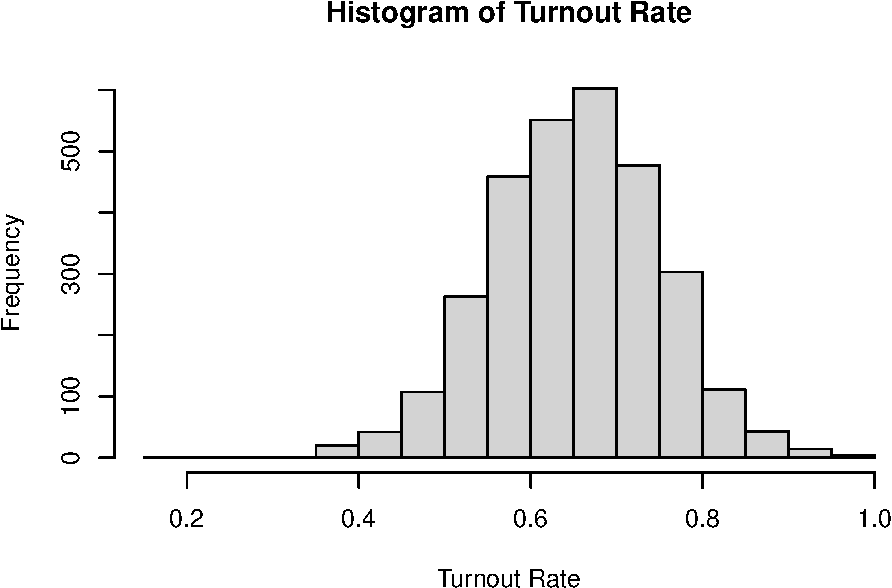
\includegraphics[keepaspectratio]{finalPaper_files/figure-latex/turnout-1.pdf}}
\caption{\label{fig:turnout}Histogram of turnout rate for counties shows an approximately normal distribution.}
\end{figure}

To see the relationship between voter turnout and one predictor variable hypothesized to be associated with it, we plot the 2010 poverty rate against the 2020 turnout rate for each county (Figure \ref{fig:povertyturnout}). There is a moderate negative association between the variables (\(r = -0.571\)).

\begin{figure}
\centering
\pandocbounded{\includegraphics[keepaspectratio]{finalPaper_files/figure-latex/povertyturnout-1.pdf}}
\caption{\label{fig:povertyturnout}Scatterplot of poverty rate vs.~turnout rate. The negative association between the two variables aligns with the theory that socioeconomic disadvantage is associated with lower electoral participation.}
\end{figure}

\section{Methods}\label{methods}

\section{Results}\label{results}

\subsection{Baseline Model}\label{baseline-model}

We first fit a simple linear regression model containing all predictors except state and no interaction terms. The model output is shown in Table \ref{tab:baseline}.

 
  \providecommand{\huxb}[2]{\arrayrulecolor[RGB]{#1}\global\arrayrulewidth=#2pt}
  \providecommand{\huxvb}[2]{\color[RGB]{#1}\vrule width #2pt}
  \providecommand{\huxtpad}[1]{\rule{0pt}{#1}}
  \providecommand{\huxbpad}[1]{\rule[-#1]{0pt}{#1}}

\begin{table}[ht]
\begin{centerbox}
\begin{threeparttable}
\setlength{\tabcolsep}{0pt}
\begin{tabular}{l l l l l}


\hhline{}
\arrayrulecolor{black}

\multicolumn{1}{!{\huxvb{0, 0, 0}{0}}l!{\huxvb{0, 0, 0}{0}}}{\huxtpad{6pt + 1em}\raggedright \hspace{6pt} \textbf{Variable
} \hspace{6pt}\huxbpad{6pt}} &
\multicolumn{1}{r!{\huxvb{0, 0, 0}{0}}}{\huxtpad{6pt + 1em}\raggedleft \hspace{6pt} \textbf{Estimate} \hspace{6pt}\huxbpad{6pt}} &
\multicolumn{1}{r!{\huxvb{0, 0, 0}{0}}}{\huxtpad{6pt + 1em}\raggedleft \hspace{6pt} \textbf{SE} \hspace{6pt}\huxbpad{6pt}} &
\multicolumn{1}{r!{\huxvb{0, 0, 0}{0}}}{\huxtpad{6pt + 1em}\raggedleft \hspace{6pt} \textbf{$t$-value} \hspace{6pt}\huxbpad{6pt}} &
\multicolumn{1}{r!{\huxvb{0, 0, 0}{0}}}{\huxtpad{6pt + 1em}\raggedleft \hspace{6pt} \textbf{$p$-value} \hspace{6pt}\huxbpad{6pt}} \tabularnewline[-0.5pt]


\hhline{>{\huxb{0, 0, 0}{1}}->{\huxb{0, 0, 0}{1}}->{\huxb{0, 0, 0}{1}}->{\huxb{0, 0, 0}{1}}->{\huxb{0, 0, 0}{1}}-}
\arrayrulecolor{black}

\multicolumn{1}{!{\huxvb{0, 0, 0}{0}}l!{\huxvb{0, 0, 0}{0}}}{\huxtpad{6pt + 1em}\raggedright \hspace{6pt} (Intercept)
 \hspace{6pt}\huxbpad{6pt}} &
\multicolumn{1}{r!{\huxvb{0, 0, 0}{0}}}{\huxtpad{6pt + 1em}\raggedleft \hspace{6pt} 0.608 \hspace{6pt}\huxbpad{6pt}} &
\multicolumn{1}{r!{\huxvb{0, 0, 0}{0}}}{\huxtpad{6pt + 1em}\raggedleft \hspace{6pt} 0.0329 \hspace{6pt}\huxbpad{6pt}} &
\multicolumn{1}{r!{\huxvb{0, 0, 0}{0}}}{\huxtpad{6pt + 1em}\raggedleft \hspace{6pt} 18.5 \hspace{6pt}\huxbpad{6pt}} &
\multicolumn{1}{r!{\huxvb{0, 0, 0}{0}}}{\huxtpad{6pt + 1em}\raggedleft \hspace{6pt} 2.4e$-$72 \hspace{6pt}\huxbpad{6pt}} \tabularnewline[-0.5pt]


\hhline{}
\arrayrulecolor{black}

\multicolumn{1}{!{\huxvb{0, 0, 0}{0}}l!{\huxvb{0, 0, 0}{0}}}{\huxtpad{6pt + 1em}\raggedright \hspace{6pt} \texttt{frac\_coll\_plus2010}
 \hspace{6pt}\huxbpad{6pt}} &
\multicolumn{1}{r!{\huxvb{0, 0, 0}{0}}}{\huxtpad{6pt + 1em}\raggedleft \hspace{6pt} 0.372 \hspace{6pt}\huxbpad{6pt}} &
\multicolumn{1}{r!{\huxvb{0, 0, 0}{0}}}{\huxtpad{6pt + 1em}\raggedleft \hspace{6pt} 0.026 \hspace{6pt}\huxbpad{6pt}} &
\multicolumn{1}{r!{\huxvb{0, 0, 0}{0}}}{\huxtpad{6pt + 1em}\raggedleft \hspace{6pt} 14.3 \hspace{6pt}\huxbpad{6pt}} &
\multicolumn{1}{r!{\huxvb{0, 0, 0}{0}}}{\huxtpad{6pt + 1em}\raggedleft \hspace{6pt} 5.44e$-$45 \hspace{6pt}\huxbpad{6pt}} \tabularnewline[-0.5pt]


\hhline{}
\arrayrulecolor{black}

\multicolumn{1}{!{\huxvb{0, 0, 0}{0}}l!{\huxvb{0, 0, 0}{0}}}{\huxtpad{6pt + 1em}\raggedright \hspace{6pt} \texttt{foreign\_share2010}
 \hspace{6pt}\huxbpad{6pt}} &
\multicolumn{1}{r!{\huxvb{0, 0, 0}{0}}}{\huxtpad{6pt + 1em}\raggedleft \hspace{6pt} 0.11 \hspace{6pt}\huxbpad{6pt}} &
\multicolumn{1}{r!{\huxvb{0, 0, 0}{0}}}{\huxtpad{6pt + 1em}\raggedleft \hspace{6pt} 0.0496 \hspace{6pt}\huxbpad{6pt}} &
\multicolumn{1}{r!{\huxvb{0, 0, 0}{0}}}{\huxtpad{6pt + 1em}\raggedleft \hspace{6pt} 2.23 \hspace{6pt}\huxbpad{6pt}} &
\multicolumn{1}{r!{\huxvb{0, 0, 0}{0}}}{\huxtpad{6pt + 1em}\raggedleft \hspace{6pt} 0.026 \hspace{6pt}\huxbpad{6pt}} \tabularnewline[-0.5pt]


\hhline{}
\arrayrulecolor{black}

\multicolumn{1}{!{\huxvb{0, 0, 0}{0}}l!{\huxvb{0, 0, 0}{0}}}{\huxtpad{6pt + 1em}\raggedright \hspace{6pt} \texttt{med\_hhinc2016}
 \hspace{6pt}\huxbpad{6pt}} &
\multicolumn{1}{r!{\huxvb{0, 0, 0}{0}}}{\huxtpad{6pt + 1em}\raggedleft \hspace{6pt} 1.3e$-$07 \hspace{6pt}\huxbpad{6pt}} &
\multicolumn{1}{r!{\huxvb{0, 0, 0}{0}}}{\huxtpad{6pt + 1em}\raggedleft \hspace{6pt} 2.54e$-$07 \hspace{6pt}\huxbpad{6pt}} &
\multicolumn{1}{r!{\huxvb{0, 0, 0}{0}}}{\huxtpad{6pt + 1em}\raggedleft \hspace{6pt} 0.51 \hspace{6pt}\huxbpad{6pt}} &
\multicolumn{1}{r!{\huxvb{0, 0, 0}{0}}}{\huxtpad{6pt + 1em}\raggedleft \hspace{6pt} 0.61 \hspace{6pt}\huxbpad{6pt}} \tabularnewline[-0.5pt]


\hhline{}
\arrayrulecolor{black}

\multicolumn{1}{!{\huxvb{0, 0, 0}{0}}l!{\huxvb{0, 0, 0}{0}}}{\huxtpad{6pt + 1em}\raggedright \hspace{6pt} \texttt{poor\_share2010}
 \hspace{6pt}\huxbpad{6pt}} &
\multicolumn{1}{r!{\huxvb{0, 0, 0}{0}}}{\huxtpad{6pt + 1em}\raggedleft \hspace{6pt} $-$0.576 \hspace{6pt}\huxbpad{6pt}} &
\multicolumn{1}{r!{\huxvb{0, 0, 0}{0}}}{\huxtpad{6pt + 1em}\raggedleft \hspace{6pt} 0.0404 \hspace{6pt}\huxbpad{6pt}} &
\multicolumn{1}{r!{\huxvb{0, 0, 0}{0}}}{\huxtpad{6pt + 1em}\raggedleft \hspace{6pt} $-$14.3 \hspace{6pt}\huxbpad{6pt}} &
\multicolumn{1}{r!{\huxvb{0, 0, 0}{0}}}{\huxtpad{6pt + 1em}\raggedleft \hspace{6pt} 1.08e$-$44 \hspace{6pt}\huxbpad{6pt}} \tabularnewline[-0.5pt]


\hhline{}
\arrayrulecolor{black}

\multicolumn{1}{!{\huxvb{0, 0, 0}{0}}l!{\huxvb{0, 0, 0}{0}}}{\huxtpad{6pt + 1em}\raggedright \hspace{6pt} \texttt{share\_white2010}
 \hspace{6pt}\huxbpad{6pt}} &
\multicolumn{1}{r!{\huxvb{0, 0, 0}{0}}}{\huxtpad{6pt + 1em}\raggedleft \hspace{6pt} 0.0423 \hspace{6pt}\huxbpad{6pt}} &
\multicolumn{1}{r!{\huxvb{0, 0, 0}{0}}}{\huxtpad{6pt + 1em}\raggedleft \hspace{6pt} 0.0208 \hspace{6pt}\huxbpad{6pt}} &
\multicolumn{1}{r!{\huxvb{0, 0, 0}{0}}}{\huxtpad{6pt + 1em}\raggedleft \hspace{6pt} 2.03 \hspace{6pt}\huxbpad{6pt}} &
\multicolumn{1}{r!{\huxvb{0, 0, 0}{0}}}{\huxtpad{6pt + 1em}\raggedleft \hspace{6pt} 0.0421 \hspace{6pt}\huxbpad{6pt}} \tabularnewline[-0.5pt]


\hhline{}
\arrayrulecolor{black}

\multicolumn{1}{!{\huxvb{0, 0, 0}{0}}l!{\huxvb{0, 0, 0}{0}}}{\huxtpad{6pt + 1em}\raggedright \hspace{6pt} \texttt{share\_black2010}
 \hspace{6pt}\huxbpad{6pt}} &
\multicolumn{1}{r!{\huxvb{0, 0, 0}{0}}}{\huxtpad{6pt + 1em}\raggedleft \hspace{6pt} 0.0591 \hspace{6pt}\huxbpad{6pt}} &
\multicolumn{1}{r!{\huxvb{0, 0, 0}{0}}}{\huxtpad{6pt + 1em}\raggedleft \hspace{6pt} 0.0208 \hspace{6pt}\huxbpad{6pt}} &
\multicolumn{1}{r!{\huxvb{0, 0, 0}{0}}}{\huxtpad{6pt + 1em}\raggedleft \hspace{6pt} 2.83 \hspace{6pt}\huxbpad{6pt}} &
\multicolumn{1}{r!{\huxvb{0, 0, 0}{0}}}{\huxtpad{6pt + 1em}\raggedleft \hspace{6pt} 0.00462 \hspace{6pt}\huxbpad{6pt}} \tabularnewline[-0.5pt]


\hhline{}
\arrayrulecolor{black}

\multicolumn{1}{!{\huxvb{0, 0, 0}{0}}l!{\huxvb{0, 0, 0}{0}}}{\huxtpad{6pt + 1em}\raggedright \hspace{6pt} \texttt{share\_hisp2010}
 \hspace{6pt}\huxbpad{6pt}} &
\multicolumn{1}{r!{\huxvb{0, 0, 0}{0}}}{\huxtpad{6pt + 1em}\raggedleft \hspace{6pt} $-$0.0511 \hspace{6pt}\huxbpad{6pt}} &
\multicolumn{1}{r!{\huxvb{0, 0, 0}{0}}}{\huxtpad{6pt + 1em}\raggedleft \hspace{6pt} 0.0249 \hspace{6pt}\huxbpad{6pt}} &
\multicolumn{1}{r!{\huxvb{0, 0, 0}{0}}}{\huxtpad{6pt + 1em}\raggedleft \hspace{6pt} $-$2.06 \hspace{6pt}\huxbpad{6pt}} &
\multicolumn{1}{r!{\huxvb{0, 0, 0}{0}}}{\huxtpad{6pt + 1em}\raggedleft \hspace{6pt} 0.0398 \hspace{6pt}\huxbpad{6pt}} \tabularnewline[-0.5pt]


\hhline{}
\arrayrulecolor{black}

\multicolumn{1}{!{\huxvb{0, 0, 0}{0}}l!{\huxvb{0, 0, 0}{0}}}{\huxtpad{6pt + 1em}\raggedright \hspace{6pt} \texttt{share\_asian2010}
 \hspace{6pt}\huxbpad{6pt}} &
\multicolumn{1}{r!{\huxvb{0, 0, 0}{0}}}{\huxtpad{6pt + 1em}\raggedleft \hspace{6pt} $-$0.506 \hspace{6pt}\huxbpad{6pt}} &
\multicolumn{1}{r!{\huxvb{0, 0, 0}{0}}}{\huxtpad{6pt + 1em}\raggedleft \hspace{6pt} 0.0917 \hspace{6pt}\huxbpad{6pt}} &
\multicolumn{1}{r!{\huxvb{0, 0, 0}{0}}}{\huxtpad{6pt + 1em}\raggedleft \hspace{6pt} $-$5.52 \hspace{6pt}\huxbpad{6pt}} &
\multicolumn{1}{r!{\huxvb{0, 0, 0}{0}}}{\huxtpad{6pt + 1em}\raggedleft \hspace{6pt} 3.71e$-$08 \hspace{6pt}\huxbpad{6pt}} \tabularnewline[-0.5pt]


\hhline{}
\arrayrulecolor{black}

\multicolumn{1}{!{\huxvb{0, 0, 0}{0}}l!{\huxvb{0, 0, 0}{0}}}{\huxtpad{6pt + 1em}\raggedright \hspace{6pt} \texttt{gsmn\_math\_g3\_2013}
 \hspace{6pt}\huxbpad{6pt}} &
\multicolumn{1}{r!{\huxvb{0, 0, 0}{0}}}{\huxtpad{6pt + 1em}\raggedleft \hspace{6pt} $-$0.000993 \hspace{6pt}\huxbpad{6pt}} &
\multicolumn{1}{r!{\huxvb{0, 0, 0}{0}}}{\huxtpad{6pt + 1em}\raggedleft \hspace{6pt} 0.00214 \hspace{6pt}\huxbpad{6pt}} &
\multicolumn{1}{r!{\huxvb{0, 0, 0}{0}}}{\huxtpad{6pt + 1em}\raggedleft \hspace{6pt} $-$0.464 \hspace{6pt}\huxbpad{6pt}} &
\multicolumn{1}{r!{\huxvb{0, 0, 0}{0}}}{\huxtpad{6pt + 1em}\raggedleft \hspace{6pt} 0.643 \hspace{6pt}\huxbpad{6pt}} \tabularnewline[-0.5pt]


\hhline{}
\arrayrulecolor{black}

\multicolumn{1}{!{\huxvb{0, 0, 0}{0}}l!{\huxvb{0, 0, 0}{0}}}{\huxtpad{6pt + 1em}\raggedright \hspace{6pt} \texttt{rent\_twobed2015}
 \hspace{6pt}\huxbpad{6pt}} &
\multicolumn{1}{r!{\huxvb{0, 0, 0}{0}}}{\huxtpad{6pt + 1em}\raggedleft \hspace{6pt} $-$7.02e$-$06 \hspace{6pt}\huxbpad{6pt}} &
\multicolumn{1}{r!{\huxvb{0, 0, 0}{0}}}{\huxtpad{6pt + 1em}\raggedleft \hspace{6pt} 1.43e$-$05 \hspace{6pt}\huxbpad{6pt}} &
\multicolumn{1}{r!{\huxvb{0, 0, 0}{0}}}{\huxtpad{6pt + 1em}\raggedleft \hspace{6pt} $-$0.492 \hspace{6pt}\huxbpad{6pt}} &
\multicolumn{1}{r!{\huxvb{0, 0, 0}{0}}}{\huxtpad{6pt + 1em}\raggedleft \hspace{6pt} 0.623 \hspace{6pt}\huxbpad{6pt}} \tabularnewline[-0.5pt]


\hhline{}
\arrayrulecolor{black}

\multicolumn{1}{!{\huxvb{0, 0, 0}{0}}l!{\huxvb{0, 0, 0}{0}}}{\huxtpad{6pt + 1em}\raggedright \hspace{6pt} \texttt{singleparent\_share2010}
 \hspace{6pt}\huxbpad{6pt}} &
\multicolumn{1}{r!{\huxvb{0, 0, 0}{0}}}{\huxtpad{6pt + 1em}\raggedleft \hspace{6pt} $-$0.0617 \hspace{6pt}\huxbpad{6pt}} &
\multicolumn{1}{r!{\huxvb{0, 0, 0}{0}}}{\huxtpad{6pt + 1em}\raggedleft \hspace{6pt} 0.0246 \hspace{6pt}\huxbpad{6pt}} &
\multicolumn{1}{r!{\huxvb{0, 0, 0}{0}}}{\huxtpad{6pt + 1em}\raggedleft \hspace{6pt} $-$2.51 \hspace{6pt}\huxbpad{6pt}} &
\multicolumn{1}{r!{\huxvb{0, 0, 0}{0}}}{\huxtpad{6pt + 1em}\raggedleft \hspace{6pt} 0.012 \hspace{6pt}\huxbpad{6pt}} \tabularnewline[-0.5pt]


\hhline{}
\arrayrulecolor{black}

\multicolumn{1}{!{\huxvb{0, 0, 0}{0}}l!{\huxvb{0, 0, 0}{0}}}{\huxtpad{6pt + 1em}\raggedright \hspace{6pt} \texttt{traveltime15\_2010}
 \hspace{6pt}\huxbpad{6pt}} &
\multicolumn{1}{r!{\huxvb{0, 0, 0}{0}}}{\huxtpad{6pt + 1em}\raggedleft \hspace{6pt} $-$0.0425 \hspace{6pt}\huxbpad{6pt}} &
\multicolumn{1}{r!{\huxvb{0, 0, 0}{0}}}{\huxtpad{6pt + 1em}\raggedleft \hspace{6pt} 0.0117 \hspace{6pt}\huxbpad{6pt}} &
\multicolumn{1}{r!{\huxvb{0, 0, 0}{0}}}{\huxtpad{6pt + 1em}\raggedleft \hspace{6pt} $-$3.63 \hspace{6pt}\huxbpad{6pt}} &
\multicolumn{1}{r!{\huxvb{0, 0, 0}{0}}}{\huxtpad{6pt + 1em}\raggedleft \hspace{6pt} 0.000283 \hspace{6pt}\huxbpad{6pt}} \tabularnewline[-0.5pt]


\hhline{}
\arrayrulecolor{black}

\multicolumn{1}{!{\huxvb{0, 0, 0}{0}}l!{\huxvb{0, 0, 0}{0}}}{\huxtpad{6pt + 1em}\raggedright \hspace{6pt} \texttt{emp2000}
 \hspace{6pt}\huxbpad{6pt}} &
\multicolumn{1}{r!{\huxvb{0, 0, 0}{0}}}{\huxtpad{6pt + 1em}\raggedleft \hspace{6pt} 0.114 \hspace{6pt}\huxbpad{6pt}} &
\multicolumn{1}{r!{\huxvb{0, 0, 0}{0}}}{\huxtpad{6pt + 1em}\raggedleft \hspace{6pt} 0.0273 \hspace{6pt}\huxbpad{6pt}} &
\multicolumn{1}{r!{\huxvb{0, 0, 0}{0}}}{\huxtpad{6pt + 1em}\raggedleft \hspace{6pt} 4.17 \hspace{6pt}\huxbpad{6pt}} &
\multicolumn{1}{r!{\huxvb{0, 0, 0}{0}}}{\huxtpad{6pt + 1em}\raggedleft \hspace{6pt} 3.17e$-$05 \hspace{6pt}\huxbpad{6pt}} \tabularnewline[-0.5pt]


\hhline{}
\arrayrulecolor{black}

\multicolumn{1}{!{\huxvb{0, 0, 0}{0}}l!{\huxvb{0, 0, 0}{0}}}{\huxtpad{6pt + 1em}\raggedright \hspace{6pt} \texttt{popdensity2010}
 \hspace{6pt}\huxbpad{6pt}} &
\multicolumn{1}{r!{\huxvb{0, 0, 0}{0}}}{\huxtpad{6pt + 1em}\raggedleft \hspace{6pt} $-$2.26e$-$07 \hspace{6pt}\huxbpad{6pt}} &
\multicolumn{1}{r!{\huxvb{0, 0, 0}{0}}}{\huxtpad{6pt + 1em}\raggedleft \hspace{6pt} 5.51e$-$06 \hspace{6pt}\huxbpad{6pt}} &
\multicolumn{1}{r!{\huxvb{0, 0, 0}{0}}}{\huxtpad{6pt + 1em}\raggedleft \hspace{6pt} $-$0.041 \hspace{6pt}\huxbpad{6pt}} &
\multicolumn{1}{r!{\huxvb{0, 0, 0}{0}}}{\huxtpad{6pt + 1em}\raggedleft \hspace{6pt} 0.967 \hspace{6pt}\huxbpad{6pt}} \tabularnewline[-0.5pt]


\hhline{}
\arrayrulecolor{black}

\multicolumn{1}{!{\huxvb{0, 0, 0}{0}}l!{\huxvb{0, 0, 0}{0}}}{\huxtpad{6pt + 1em}\raggedright \hspace{6pt} \texttt{ann\_avg\_job\_growth\_2004\_2013}
 \hspace{6pt}\huxbpad{6pt}} &
\multicolumn{1}{r!{\huxvb{0, 0, 0}{0}}}{\huxtpad{6pt + 1em}\raggedleft \hspace{6pt} $-$0.707 \hspace{6pt}\huxbpad{6pt}} &
\multicolumn{1}{r!{\huxvb{0, 0, 0}{0}}}{\huxtpad{6pt + 1em}\raggedleft \hspace{6pt} 0.107 \hspace{6pt}\huxbpad{6pt}} &
\multicolumn{1}{r!{\huxvb{0, 0, 0}{0}}}{\huxtpad{6pt + 1em}\raggedleft \hspace{6pt} $-$6.62 \hspace{6pt}\huxbpad{6pt}} &
\multicolumn{1}{r!{\huxvb{0, 0, 0}{0}}}{\huxtpad{6pt + 1em}\raggedleft \hspace{6pt} 4.12e$-$11 \hspace{6pt}\huxbpad{6pt}} \tabularnewline[-0.5pt]


\hhline{}
\arrayrulecolor{black}

\multicolumn{1}{!{\huxvb{0, 0, 0}{0}}l!{\huxvb{0, 0, 0}{0}}}{\huxtpad{6pt + 1em}\raggedright \hspace{6pt} \texttt{job\_density\_2013}
 \hspace{6pt}\huxbpad{6pt}} &
\multicolumn{1}{r!{\huxvb{0, 0, 0}{0}}}{\huxtpad{6pt + 1em}\raggedleft \hspace{6pt} $-$4.92e$-$06 \hspace{6pt}\huxbpad{6pt}} &
\multicolumn{1}{r!{\huxvb{0, 0, 0}{0}}}{\huxtpad{6pt + 1em}\raggedleft \hspace{6pt} 1.13e$-$05 \hspace{6pt}\huxbpad{6pt}} &
\multicolumn{1}{r!{\huxvb{0, 0, 0}{0}}}{\huxtpad{6pt + 1em}\raggedleft \hspace{6pt} $-$0.434 \hspace{6pt}\huxbpad{6pt}} &
\multicolumn{1}{r!{\huxvb{0, 0, 0}{0}}}{\huxtpad{6pt + 1em}\raggedleft \hspace{6pt} 0.665 \hspace{6pt}\huxbpad{6pt}} \tabularnewline[-0.5pt]


\hhline{}
\arrayrulecolor{black}
\end{tabular}\captionsetup{justification=centering,singlelinecheck=off}
\caption{\label{tab:baseline} Baseline model output.}
 
\end{threeparttable}\par\end{centerbox}

\end{table}
 

The baseline model demonstrates several significant relationships. The model explains approximately 44\% of the variance in turnout rates (\(R^2 = 0.442\)). Education emerges as a strong positive predictor, with a one percentage point increase in college education associated with a \(0.372\) percentage point increase in turnout (\(p < 0.001\)). Other significant positive predictors include foreign-born share (\(\hat{\beta} = 0.110\)), White population share (\(\hat{\beta} = 0.042\)), Black population share (\(\hat{\beta} = 0.059\)), and employment (\(\hat{\beta} = 0.114\)). Several factors show significant negative associations with turnout: poverty rate exhibits a strong negative effect (\(\hat{\beta} = -0.576\)), as do Hispanic population share (\(\hat{\beta} = -0.051\)), Asian population share (\(\hat{\beta} = -0.506\)), single parent share (\(\hat{\beta} = -0.062\)), travel time (\(\hat{\beta} = -0.043\)), and job growth (\(\hat{\beta} = -0.707\)). Lastly, several variables, including median household income, math scores, two-bedroom rent, population density, and job density, are not significantly related to turnout at the \(\alpha = 0.05\) threshold. This initial exploration suggests that socioeconomic
conditions significantly shape local electoral participation.

\subsubsection{Diagnostics}\label{diagnostics}

We conduct diagnostics for the baseline model to assess its suitability for linear regression. Below we assess the assumptions required for OLS linear regression:

\begin{itemize}
\tightlist
\item
  \textbf{Existence of Variance:} Residuals are reasonably dispersed, confirming the existence of variation in
  the dependent variable.
\item
  \textbf{Linearity:} The residuals vs.~fitted values plot (Figure \ref{fig:diagnostics}a) does not show pronounced curvature, suggesting linearity is generally satisfied.
\item
  \textbf{Independence:} Spatial correlation may exist between neighboring counties; external tests (like Moran's I) should be considered for future analyses.
\item
  \textbf{Homogeneity (Homoscedasticity):} Some fanning in the residuals vs.~fitted values plot (Figure \ref{fig:diagnostics}a) suggests heteroscedasticity. Robust standard errors or alternative modeling approaches may be warranted.
\item
  \textbf{Normality:} The Q-Q plot (Figure \ref{fig:diagnostics}b) shows mostly normal residuals, with minor deviations in the tails.
\end{itemize}

Overall, while the model is a decent fit, improvements---such as using robust errors or accounting for spatial autocorrelation---could refine our inference.

\begin{figure}
\subfloat[Residuals vs. fitted values plot.\label{fig:diagnostics-1}]{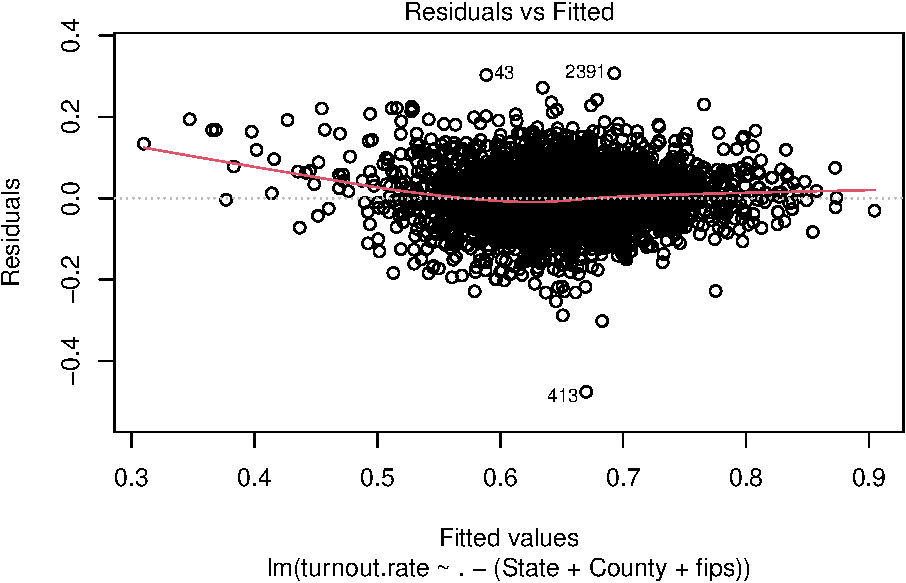
\includegraphics[width=.49\linewidth]{finalPaper_files/figure-latex/diagnostics-1} }\subfloat[Q-Q residual plot.\label{fig:diagnostics-2}]{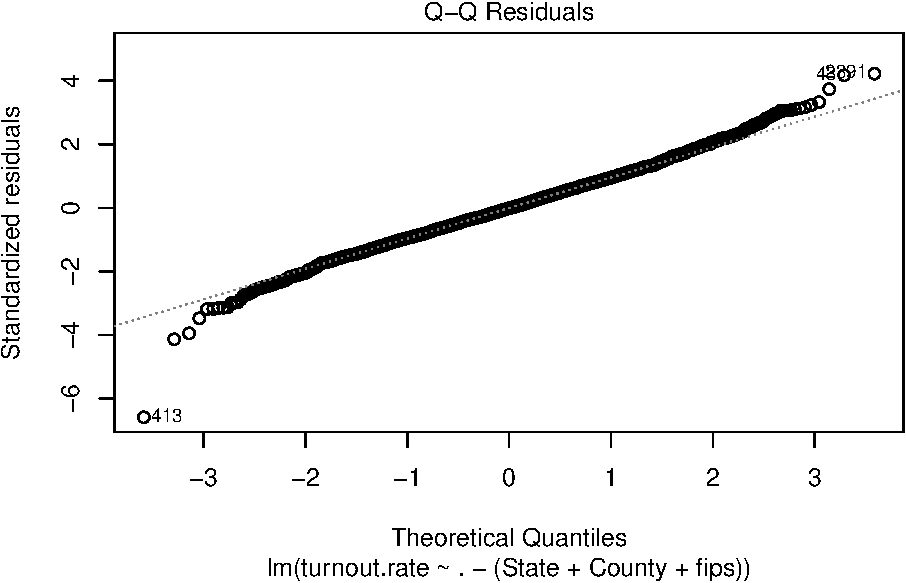
\includegraphics[width=.49\linewidth]{finalPaper_files/figure-latex/diagnostics-2} }\caption{Diagnostic plots for baseline model.}\label{fig:diagnostics}
\end{figure}

\subsection{Regularization}\label{regularization}

To address potential overfitting and identify the most influential variables, we employ LASSO regularization, which introduces a penalty that can shrink some coefficients to zero.

\textcolor{red}{Elaborate on LASSO}

 
  \providecommand{\huxb}[2]{\arrayrulecolor[RGB]{#1}\global\arrayrulewidth=#2pt}
  \providecommand{\huxvb}[2]{\color[RGB]{#1}\vrule width #2pt}
  \providecommand{\huxtpad}[1]{\rule{0pt}{#1}}
  \providecommand{\huxbpad}[1]{\rule[-#1]{0pt}{#1}}

\begin{table}[ht]
\begin{centerbox}
\begin{threeparttable}
\setlength{\tabcolsep}{0pt}
\begin{tabular}{l l}


\hhline{}
\arrayrulecolor{black}

\multicolumn{1}{!{\huxvb{0, 0, 0}{0}}l!{\huxvb{0, 0, 0}{0}}}{\huxtpad{6pt + 1em}\raggedright \hspace{6pt} \textbf{Variable
} \hspace{6pt}\huxbpad{6pt}} &
\multicolumn{1}{r!{\huxvb{0, 0, 0}{0}}}{\huxtpad{6pt + 1em}\raggedleft \hspace{6pt} \textbf{Coefficient} \hspace{6pt}\huxbpad{6pt}} \tabularnewline[-0.5pt]


\hhline{>{\huxb{0, 0, 0}{1}}->{\huxb{0, 0, 0}{1}}-}
\arrayrulecolor{black}

\multicolumn{1}{!{\huxvb{0, 0, 0}{0}}l!{\huxvb{0, 0, 0}{0}}}{\huxtpad{6pt + 1em}\raggedright \hspace{6pt} (Intercept)
 \hspace{6pt}\huxbpad{6pt}} &
\multicolumn{1}{r!{\huxvb{0, 0, 0}{0}}}{\huxtpad{6pt + 1em}\raggedleft \hspace{6pt} 0.612 \hspace{6pt}\huxbpad{6pt}} \tabularnewline[-0.5pt]


\hhline{}
\arrayrulecolor{black}

\multicolumn{1}{!{\huxvb{0, 0, 0}{0}}l!{\huxvb{0, 0, 0}{0}}}{\huxtpad{6pt + 1em}\raggedright \hspace{6pt} \texttt{frac\_coll\_plus2010}
 \hspace{6pt}\huxbpad{6pt}} &
\multicolumn{1}{r!{\huxvb{0, 0, 0}{0}}}{\huxtpad{6pt + 1em}\raggedleft \hspace{6pt} 0.363 \hspace{6pt}\huxbpad{6pt}} \tabularnewline[-0.5pt]


\hhline{}
\arrayrulecolor{black}

\multicolumn{1}{!{\huxvb{0, 0, 0}{0}}l!{\huxvb{0, 0, 0}{0}}}{\huxtpad{6pt + 1em}\raggedright \hspace{6pt} \texttt{foreign\_share2010}
 \hspace{6pt}\huxbpad{6pt}} &
\multicolumn{1}{r!{\huxvb{0, 0, 0}{0}}}{\huxtpad{6pt + 1em}\raggedleft \hspace{6pt} 0.0702 \hspace{6pt}\huxbpad{6pt}} \tabularnewline[-0.5pt]


\hhline{}
\arrayrulecolor{black}

\multicolumn{1}{!{\huxvb{0, 0, 0}{0}}l!{\huxvb{0, 0, 0}{0}}}{\huxtpad{6pt + 1em}\raggedright \hspace{6pt} \texttt{med\_hhinc2016}
 \hspace{6pt}\huxbpad{6pt}} &
\multicolumn{1}{r!{\huxvb{0, 0, 0}{0}}}{\huxtpad{6pt + 1em}\raggedleft \hspace{6pt} 4.44e$-$08 \hspace{6pt}\huxbpad{6pt}} \tabularnewline[-0.5pt]


\hhline{}
\arrayrulecolor{black}

\multicolumn{1}{!{\huxvb{0, 0, 0}{0}}l!{\huxvb{0, 0, 0}{0}}}{\huxtpad{6pt + 1em}\raggedright \hspace{6pt} \texttt{poor\_share2010}
 \hspace{6pt}\huxbpad{6pt}} &
\multicolumn{1}{r!{\huxvb{0, 0, 0}{0}}}{\huxtpad{6pt + 1em}\raggedleft \hspace{6pt} $-$0.574 \hspace{6pt}\huxbpad{6pt}} \tabularnewline[-0.5pt]


\hhline{}
\arrayrulecolor{black}

\multicolumn{1}{!{\huxvb{0, 0, 0}{0}}l!{\huxvb{0, 0, 0}{0}}}{\huxtpad{6pt + 1em}\raggedright \hspace{6pt} \texttt{share\_white2010}
 \hspace{6pt}\huxbpad{6pt}} &
\multicolumn{1}{r!{\huxvb{0, 0, 0}{0}}}{\huxtpad{6pt + 1em}\raggedleft \hspace{6pt} 0.0339 \hspace{6pt}\huxbpad{6pt}} \tabularnewline[-0.5pt]


\hhline{}
\arrayrulecolor{black}

\multicolumn{1}{!{\huxvb{0, 0, 0}{0}}l!{\huxvb{0, 0, 0}{0}}}{\huxtpad{6pt + 1em}\raggedright \hspace{6pt} \texttt{share\_black2010}
 \hspace{6pt}\huxbpad{6pt}} &
\multicolumn{1}{r!{\huxvb{0, 0, 0}{0}}}{\huxtpad{6pt + 1em}\raggedleft \hspace{6pt} 0.0499 \hspace{6pt}\huxbpad{6pt}} \tabularnewline[-0.5pt]


\hhline{}
\arrayrulecolor{black}

\multicolumn{1}{!{\huxvb{0, 0, 0}{0}}l!{\huxvb{0, 0, 0}{0}}}{\huxtpad{6pt + 1em}\raggedright \hspace{6pt} \texttt{share\_hisp2010}
 \hspace{6pt}\huxbpad{6pt}} &
\multicolumn{1}{r!{\huxvb{0, 0, 0}{0}}}{\huxtpad{6pt + 1em}\raggedleft \hspace{6pt} $-$0.0486 \hspace{6pt}\huxbpad{6pt}} \tabularnewline[-0.5pt]


\hhline{}
\arrayrulecolor{black}

\multicolumn{1}{!{\huxvb{0, 0, 0}{0}}l!{\huxvb{0, 0, 0}{0}}}{\huxtpad{6pt + 1em}\raggedright \hspace{6pt} \texttt{share\_asian2010}
 \hspace{6pt}\huxbpad{6pt}} &
\multicolumn{1}{r!{\huxvb{0, 0, 0}{0}}}{\huxtpad{6pt + 1em}\raggedleft \hspace{6pt} $-$0.47 \hspace{6pt}\huxbpad{6pt}} \tabularnewline[-0.5pt]


\hhline{}
\arrayrulecolor{black}

\multicolumn{1}{!{\huxvb{0, 0, 0}{0}}l!{\huxvb{0, 0, 0}{0}}}{\huxtpad{6pt + 1em}\raggedright \hspace{6pt} \texttt{gsmn\_math\_g3\_2013}
 \hspace{6pt}\huxbpad{6pt}} &
\multicolumn{1}{r!{\huxvb{0, 0, 0}{0}}}{\huxtpad{6pt + 1em}\raggedleft \hspace{6pt} 0 \hspace{6pt}\huxbpad{6pt}} \tabularnewline[-0.5pt]


\hhline{}
\arrayrulecolor{black}

\multicolumn{1}{!{\huxvb{0, 0, 0}{0}}l!{\huxvb{0, 0, 0}{0}}}{\huxtpad{6pt + 1em}\raggedright \hspace{6pt} \texttt{rent\_twobed2015}
 \hspace{6pt}\huxbpad{6pt}} &
\multicolumn{1}{r!{\huxvb{0, 0, 0}{0}}}{\huxtpad{6pt + 1em}\raggedleft \hspace{6pt} 0 \hspace{6pt}\huxbpad{6pt}} \tabularnewline[-0.5pt]


\hhline{}
\arrayrulecolor{black}

\multicolumn{1}{!{\huxvb{0, 0, 0}{0}}l!{\huxvb{0, 0, 0}{0}}}{\huxtpad{6pt + 1em}\raggedright \hspace{6pt} \texttt{singleparent\_share2010}
 \hspace{6pt}\huxbpad{6pt}} &
\multicolumn{1}{r!{\huxvb{0, 0, 0}{0}}}{\huxtpad{6pt + 1em}\raggedleft \hspace{6pt} $-$0.0605 \hspace{6pt}\huxbpad{6pt}} \tabularnewline[-0.5pt]


\hhline{}
\arrayrulecolor{black}

\multicolumn{1}{!{\huxvb{0, 0, 0}{0}}l!{\huxvb{0, 0, 0}{0}}}{\huxtpad{6pt + 1em}\raggedright \hspace{6pt} \texttt{traveltime15\_2010}
 \hspace{6pt}\huxbpad{6pt}} &
\multicolumn{1}{r!{\huxvb{0, 0, 0}{0}}}{\huxtpad{6pt + 1em}\raggedleft \hspace{6pt} $-$0.0412 \hspace{6pt}\huxbpad{6pt}} \tabularnewline[-0.5pt]


\hhline{}
\arrayrulecolor{black}

\multicolumn{1}{!{\huxvb{0, 0, 0}{0}}l!{\huxvb{0, 0, 0}{0}}}{\huxtpad{6pt + 1em}\raggedright \hspace{6pt} \texttt{emp2000}
 \hspace{6pt}\huxbpad{6pt}} &
\multicolumn{1}{r!{\huxvb{0, 0, 0}{0}}}{\huxtpad{6pt + 1em}\raggedleft \hspace{6pt} 0.116 \hspace{6pt}\huxbpad{6pt}} \tabularnewline[-0.5pt]


\hhline{}
\arrayrulecolor{black}

\multicolumn{1}{!{\huxvb{0, 0, 0}{0}}l!{\huxvb{0, 0, 0}{0}}}{\huxtpad{6pt + 1em}\raggedright \hspace{6pt} \texttt{popdensity2010}
 \hspace{6pt}\huxbpad{6pt}} &
\multicolumn{1}{r!{\huxvb{0, 0, 0}{0}}}{\huxtpad{6pt + 1em}\raggedleft \hspace{6pt} $-$8.43e$-$07 \hspace{6pt}\huxbpad{6pt}} \tabularnewline[-0.5pt]


\hhline{}
\arrayrulecolor{black}

\multicolumn{1}{!{\huxvb{0, 0, 0}{0}}l!{\huxvb{0, 0, 0}{0}}}{\huxtpad{6pt + 1em}\raggedright \hspace{6pt} \texttt{ann\_avg\_job\_growth\_2004\_2013}
 \hspace{6pt}\huxbpad{6pt}} &
\multicolumn{1}{r!{\huxvb{0, 0, 0}{0}}}{\huxtpad{6pt + 1em}\raggedleft \hspace{6pt} $-$0.67 \hspace{6pt}\huxbpad{6pt}} \tabularnewline[-0.5pt]


\hhline{}
\arrayrulecolor{black}

\multicolumn{1}{!{\huxvb{0, 0, 0}{0}}l!{\huxvb{0, 0, 0}{0}}}{\huxtpad{6pt + 1em}\raggedright \hspace{6pt} \texttt{job\_density\_2013}
 \hspace{6pt}\huxbpad{6pt}} &
\multicolumn{1}{r!{\huxvb{0, 0, 0}{0}}}{\huxtpad{6pt + 1em}\raggedleft \hspace{6pt} $-$3.17e$-$06 \hspace{6pt}\huxbpad{6pt}} \tabularnewline[-0.5pt]


\hhline{}
\arrayrulecolor{black}
\end{tabular}\captionsetup{justification=centering,singlelinecheck=off}
\caption{\label{tab:lasso} Coefficients after LASSO regularization with $\lambda = 2.769\mathrm{e-}4$.}
 
\end{threeparttable}\par\end{centerbox}

\end{table}
 

The optimal \(\lambda = 2.769\mathrm{e-}4\) was selected through ten-fold cross-validation to achieve a penalty level that balances predictive accuracy and model complexity. This approach ensures we do not overfit by including too many small-effect predictors.

\begin{figure}
\centering
\pandocbounded{\includegraphics[keepaspectratio]{finalPaper_files/figure-latex/lassoplot-1.pdf}}
\caption{\label{fig:lassoplot}CAPTION!}
\end{figure}

As \(\lambda\) increases (moving right on the \(x\)-axis of Figure \ref{fig:lassoplot}), the regularization strength increases and more predictors drop out of the model with coefficients of 0. The vertical dashed black line shows the chosen \(\lambda\). Predictors with coefficients of 0 at the vertical line are dropped from the final model. This graph visually demonstrates which variables are ``important enough'' to survive the LASSO penalty.

\textcolor{red}{Not much regularization for most variables}

LASSO retained most predictors but excluded \texttt{gsmn\_math\_g3\_2013} and \texttt{rent\_twobed2015} (Table \ref{tab:lasso}). This aligns with earlier findings that these variables were not statistically significant in the preliminary linear model.

\subsection{Correlation Structure}\label{correlation-structure}

Examining correlations among predictors helps identify potential multicollinearity and structure in the data.

\begin{figure}
\centering
\pandocbounded{\includegraphics[keepaspectratio]{finalPaper_files/figure-latex/corr-1.pdf}}
\caption{\label{fig:corr}CAPTION!}
\end{figure}

The heatmap shows groups of variables that cluster together, indicating underlying socioeconomic dimensions (e.g., poverty and race-related measures clustered together, economic growth and density measures in another cluster). These clusters may reflect underlying latent factors that shape voter turnout.

One concern shown in the correlation matrix is the very high correlation between population density and job density

\subsection{Interaction Terms}\label{interaction-terms}

We test whether adding an interaction term between education and poverty (\texttt{frac\_coll\_plus2010:poor\_share2010}) improves model performance.

A highly significant test result (\(p < 2.2\mathrm{e-}16\)) suggests the interaction between college education fraction and poverty
share is crucial, indicating that the effect of education on turnout may depend on the poverty context of the
county (and vice versa).

\subsection{Final Model Including State Fixed Effects}\label{final-model-including-state-fixed-effects}

We run a final model excluding the variables zeroed out by LASSO and adding state fixed effects to control
for unobserved state-level heterogeneity.

\begin{verbatim}
## 
## Call:
## lm(formula = turnout.rate ~ . - State - County - fips - gsmn_math_g3_2013 - 
##     rent_twobed2015 + factor(State), data = data)
## 
## Residuals:
##      Min       1Q   Median       3Q      Max 
## -0.42729 -0.03049 -0.00122  0.03066  0.29353 
## 
## Coefficients:
##                                     Estimate Std. Error t value Pr(>|t|)    
## (Intercept)                        5.336e-01  2.979e-02  17.912  < 2e-16 ***
## frac_coll_plus2010                 2.398e-01  2.109e-02  11.373  < 2e-16 ***
## foreign_share2010                 -5.603e-02  4.458e-02  -1.257 0.208914    
## med_hhinc2016                      9.682e-07  2.088e-07   4.636 3.70e-06 ***
## poor_share2010                    -3.474e-01  3.486e-02  -9.966  < 2e-16 ***
## share_white2010                    9.735e-02  1.979e-02   4.918 9.21e-07 ***
## share_black2010                    1.042e-01  2.123e-02   4.908 9.73e-07 ***
## share_hisp2010                     3.103e-03  2.489e-02   0.125 0.900789    
## share_asian2010                   -5.204e-01  9.504e-02  -5.476 4.72e-08 ***
## singleparent_share2010            -8.936e-02  2.048e-02  -4.363 1.32e-05 ***
## traveltime15_2010                 -9.101e-02  1.159e-02  -7.851 5.76e-15 ***
## emp2000                            1.104e-01  2.520e-02   4.382 1.22e-05 ***
## popdensity2010                     5.026e-06  4.507e-06   1.115 0.264946    
## ann_avg_job_growth_2004_2013      -6.982e-01  9.184e-02  -7.603 3.88e-14 ***
## job_density_2013                  -1.071e-05  9.239e-06  -1.159 0.246589    
## factor(State)Alaska                1.608e-02  1.842e-02   0.873 0.382787    
## factor(State)Arizona               5.215e-02  1.747e-02   2.985 0.002861 ** 
## factor(State)Arkansas             -9.944e-02  9.917e-03 -10.027  < 2e-16 ***
## factor(State)California            4.921e-02  1.212e-02   4.062 5.00e-05 ***
## factor(State)Colorado              8.884e-02  1.148e-02   7.740 1.36e-14 ***
## factor(State)Connecticut          -4.244e-02  2.227e-02  -1.905 0.056830 .  
## factor(State)Delaware              2.913e-03  3.433e-02   0.085 0.932388    
## factor(State)District of Columbia -4.882e-02  5.958e-02  -0.819 0.412677    
## factor(State)Florida               4.820e-02  1.050e-02   4.591 4.61e-06 ***
## factor(State)Georgia              -1.941e-02  8.546e-03  -2.271 0.023205 *  
## factor(State)Hawaii                1.088e-01  3.992e-02   2.726 0.006444 ** 
## factor(State)Idaho                 4.300e-02  1.206e-02   3.566 0.000368 ***
## factor(State)Illinois             -2.579e-02  9.701e-03  -2.658 0.007893 ** 
## factor(State)Indiana              -7.224e-02  9.951e-03  -7.259 4.97e-13 ***
## factor(State)Iowa                  3.768e-02  1.008e-02   3.738 0.000189 ***
## factor(State)Kansas               -1.577e-02  1.011e-02  -1.560 0.118888    
## factor(State)Kentucky             -1.587e-02  9.438e-03  -1.682 0.092771 .  
## factor(State)Louisiana             1.088e-03  1.026e-02   0.106 0.915566    
## factor(State)Maine                 7.530e-02  1.659e-02   4.539 5.89e-06 ***
## factor(State)Maryland             -4.177e-02  1.432e-02  -2.918 0.003554 ** 
## factor(State)Massachusetts         2.107e-02  1.785e-02   1.181 0.237859    
## factor(State)Michigan              5.593e-02  1.006e-02   5.561 2.93e-08 ***
## factor(State)Minnesota             6.894e-02  1.032e-02   6.682 2.81e-11 ***
## factor(State)Mississippi           1.263e-03  9.723e-03   0.130 0.896657    
## factor(State)Missouri             -3.106e-02  9.426e-03  -3.295 0.000997 ***
## factor(State)Montana               7.623e-02  1.243e-02   6.133 9.75e-10 ***
## factor(State)Nebraska              2.503e-02  1.080e-02   2.318 0.020507 *  
## factor(State)Nevada                5.369e-02  1.873e-02   2.866 0.004183 ** 
## factor(State)New Hampshire         6.395e-03  2.012e-02   0.318 0.750609    
## factor(State)New Jersey            2.675e-02  1.563e-02   1.711 0.087174 .  
## factor(State)New Mexico            2.117e-02  1.497e-02   1.414 0.157338    
## factor(State)New York             -5.491e-02  1.112e-02  -4.939 8.30e-07 ***
## factor(State)North Carolina        4.468e-02  9.253e-03   4.829 1.44e-06 ***
## factor(State)North Dakota         -1.759e-03  1.251e-02  -0.141 0.888178    
## factor(State)Ohio                 -2.654e-02  9.949e-03  -2.668 0.007670 ** 
## factor(State)Oklahoma             -8.357e-02  1.053e-02  -7.934 2.99e-15 ***
## factor(State)Oregon                1.182e-01  1.286e-02   9.191  < 2e-16 ***
## factor(State)Pennsylvania         -1.508e-02  1.052e-02  -1.433 0.152074    
## factor(State)Rhode Island         -5.543e-02  2.740e-02  -2.023 0.043192 *  
## factor(State)South Carolina        9.969e-04  1.132e-02   0.088 0.929836    
## factor(State)South Dakota          3.214e-03  1.180e-02   0.273 0.785250    
## factor(State)Tennessee            -6.913e-02  9.586e-03  -7.211 7.02e-13 ***
## factor(State)Texas                -2.023e-02  9.300e-03  -2.175 0.029692 *  
## factor(State)Utah                  4.048e-02  1.402e-02   2.888 0.003910 ** 
## factor(State)Vermont               3.112e-02  1.812e-02   1.718 0.085953 .  
## factor(State)Virginia              6.502e-03  8.997e-03   0.723 0.469910    
## factor(State)Washington            1.113e-01  1.247e-02   8.924  < 2e-16 ***
## factor(State)West Virginia        -8.496e-02  1.108e-02  -7.668 2.35e-14 ***
## factor(State)Wisconsin             5.134e-02  1.060e-02   4.841 1.36e-06 ***
## factor(State)Wyoming              -9.239e-03  1.497e-02  -0.617 0.537151    
## ---
## Signif. codes:  0 '***' 0.001 '**' 0.01 '*' 0.05 '.' 0.1 ' ' 1
## 
## Residual standard error: 0.058 on 2934 degrees of freedom
## Multiple R-squared:  0.6536, Adjusted R-squared:  0.646 
## F-statistic: 86.49 on 64 and 2934 DF,  p-value: < 2.2e-16
\end{verbatim}

With state fixed effects, the adjusted \(R^2\) improves to approximately 0.646, suggesting that differences between states
explain a significant portion of turnout variation. After controlling for state-level factors, education, poverty,
and various demographic characteristics remain significant. Notably, poverty and time-to-work remain
negatively associated with turnout, while educational attainment consistently shows a positive association.
This final specification suggests that while local socioeconomic conditions are important, broader state-level
contexts also shape the electoral participation landscape.

\section{Discussion and Conclusion}\label{discussion-and-conclusion}

Our analysis shows that socioeconomic and demographic factors strongly influence county-level voter turnout. Education and certain demographic features (e.g., Black population share) are robust, positive predictors of turnout, while higher poverty rates, longer travel times, and certain population characteristics (e.g., Asian population share) are negatively associated. LASSO regularization supports the exclusion of non-influential predictors, refining the model and reinforcing the significance of key variables. Incorporating interaction terms and state fixed effects further refines our understanding, revealing that the influence of education on turnout may be contingent on the economic context and that state-level factors account for substantial variation across the U.S. counties.

There are some limitations to our findings. One important caveat is that these associations between county-wide factors and voter turnout do not imply anything about the individuals within counties. Concluding that, for instance, highly educated people are more likely to vote solely based on the data presented here would an example of the ecological fallacy, where inferences about individuals are made based on inferences about groups containing those individuals (Freedman 1999). Another limitation is that there is a somewhat arbitrary time lag between the measurement of the predictors and the outcome (the socioeconomic and demographic factors are measured between 2000 and 2016, but the voter turnout rate is measured in 2020). Regardless, these findings have implications for policymakers and organizations interested in increasing voter participation. Interventions that improve socioeconomic conditions, reduce poverty, enhance education, and consider unique state-level political climates could foster higher electoral engagement, but more research should be done at the individual level or experimental level to reach more statistically sound conclusions.

\section{Bibliography}\label{bibliography}

\phantomsection\label{refs}
\begin{CSLReferences}{1}{0}
\bibitem[\citeproctext]{ref-chetty_replication_2022}
Chetty, Raj, John Friedman, Nathaniel Hendren, Maggie R. Jones, and Sonya R. Porter. 2022. {``Replication {Data} for: {The} {Opportunity} {Atlas}: {Mapping} the {Childhood} {Roots} of {Social} {Mobility}.''} Harvard Dataverse. \url{https://doi.org/10.7910/DVN/NKCQM1}.

\bibitem[\citeproctext]{ref-cinyc_alaska_2021}
cinyc. 2021. {``Alaska {Presidential} {Results} by {County} {Equivalent}, 1960-2020.''} \emph{RRH Elections}. \url{https://rrhelections.com/index.php/2021/04/13/alaska-presidential-results-by-county-equivalent-1960-2020/9/}.

\bibitem[\citeproctext]{ref-freedman_ecological_1999}
Freedman, David. 1999. {``Ecological {Inference} and the {Ecological} {Fallacy}.''} \emph{International Encyclopedia of the Social \& Behavioral Sciences} 6 (4027-4030): 1--7.

\bibitem[\citeproctext]{ref-mit_election_data_and_science_lab_county_2018}
MIT Election Data and Science Lab. 2018. {``County {Presidential} {Election} {Returns} 2000-2020.''} Harvard Dataverse. \url{https://doi.org/10.7910/DVN/VOQCHQ}.

\bibitem[\citeproctext]{ref-us_census_bureau_b05003_2020}
US Census Bureau. 2020. {``B05003: {Sex} by {Age} by {Nativity} and {Citizenship} {Status}.''} \url{https://data.census.gov/table/ACSDT5Y2020.B05003?t=Citizenship&g=010XX00US$0500000&y=2020&d=ACS\%205-Year\%20Estimates\%20Detailed\%20Tables&moe=false&tp=true}.

\bibitem[\citeproctext]{ref-us_census_bureau_american_2023}
---------. 2023. {``American {National} {Standards} {Institute} ({ANSI}), {Federal} {Information} {Processing} {Series} ({FIPS}), and {Other} {Standardized} {Geographic} {Codes}.''} \emph{Census.gov}. \url{https://www.census.gov/library/reference/code-lists/ansi.html}.

\end{CSLReferences}

\section{Appendix}\label{appendix}

\end{document}
